% Options for packages loaded elsewhere
\PassOptionsToPackage{unicode}{hyperref}
\PassOptionsToPackage{hyphens}{url}
%
\documentclass[
  english,
  man]{apa6}
\usepackage{lmodern}
\usepackage{amssymb,amsmath}
\usepackage{ifxetex,ifluatex}
\ifnum 0\ifxetex 1\fi\ifluatex 1\fi=0 % if pdftex
  \usepackage[T1]{fontenc}
  \usepackage[utf8]{inputenc}
  \usepackage{textcomp} % provide euro and other symbols
\else % if luatex or xetex
  \usepackage{unicode-math}
  \defaultfontfeatures{Scale=MatchLowercase}
  \defaultfontfeatures[\rmfamily]{Ligatures=TeX,Scale=1}
\fi
% Use upquote if available, for straight quotes in verbatim environments
\IfFileExists{upquote.sty}{\usepackage{upquote}}{}
\IfFileExists{microtype.sty}{% use microtype if available
  \usepackage[]{microtype}
  \UseMicrotypeSet[protrusion]{basicmath} % disable protrusion for tt fonts
}{}
\makeatletter
\@ifundefined{KOMAClassName}{% if non-KOMA class
  \IfFileExists{parskip.sty}{%
    \usepackage{parskip}
  }{% else
    \setlength{\parindent}{0pt}
    \setlength{\parskip}{6pt plus 2pt minus 1pt}}
}{% if KOMA class
  \KOMAoptions{parskip=half}}
\makeatother
\usepackage{xcolor}
\IfFileExists{xurl.sty}{\usepackage{xurl}}{} % add URL line breaks if available
\IfFileExists{bookmark.sty}{\usepackage{bookmark}}{\usepackage{hyperref}}
\hypersetup{
  pdftitle={The Actor-Partner Effect of Gender, Telework and Perceived Chore Fairness on Relationship Satisfaction Among Couples},
  pdfauthor={Iris Zhong1 \& Yena Li1},
  pdflang={en-EN},
  pdfkeywords={keywords},
  hidelinks,
  pdfcreator={LaTeX via pandoc}}
\urlstyle{same} % disable monospaced font for URLs
\usepackage{color}
\usepackage{fancyvrb}
\newcommand{\VerbBar}{|}
\newcommand{\VERB}{\Verb[commandchars=\\\{\}]}
\DefineVerbatimEnvironment{Highlighting}{Verbatim}{commandchars=\\\{\}}
% Add ',fontsize=\small' for more characters per line
\usepackage{framed}
\definecolor{shadecolor}{RGB}{248,248,248}
\newenvironment{Shaded}{\begin{snugshade}}{\end{snugshade}}
\newcommand{\AlertTok}[1]{\textcolor[rgb]{0.94,0.16,0.16}{#1}}
\newcommand{\AnnotationTok}[1]{\textcolor[rgb]{0.56,0.35,0.01}{\textbf{\textit{#1}}}}
\newcommand{\AttributeTok}[1]{\textcolor[rgb]{0.77,0.63,0.00}{#1}}
\newcommand{\BaseNTok}[1]{\textcolor[rgb]{0.00,0.00,0.81}{#1}}
\newcommand{\BuiltInTok}[1]{#1}
\newcommand{\CharTok}[1]{\textcolor[rgb]{0.31,0.60,0.02}{#1}}
\newcommand{\CommentTok}[1]{\textcolor[rgb]{0.56,0.35,0.01}{\textit{#1}}}
\newcommand{\CommentVarTok}[1]{\textcolor[rgb]{0.56,0.35,0.01}{\textbf{\textit{#1}}}}
\newcommand{\ConstantTok}[1]{\textcolor[rgb]{0.00,0.00,0.00}{#1}}
\newcommand{\ControlFlowTok}[1]{\textcolor[rgb]{0.13,0.29,0.53}{\textbf{#1}}}
\newcommand{\DataTypeTok}[1]{\textcolor[rgb]{0.13,0.29,0.53}{#1}}
\newcommand{\DecValTok}[1]{\textcolor[rgb]{0.00,0.00,0.81}{#1}}
\newcommand{\DocumentationTok}[1]{\textcolor[rgb]{0.56,0.35,0.01}{\textbf{\textit{#1}}}}
\newcommand{\ErrorTok}[1]{\textcolor[rgb]{0.64,0.00,0.00}{\textbf{#1}}}
\newcommand{\ExtensionTok}[1]{#1}
\newcommand{\FloatTok}[1]{\textcolor[rgb]{0.00,0.00,0.81}{#1}}
\newcommand{\FunctionTok}[1]{\textcolor[rgb]{0.00,0.00,0.00}{#1}}
\newcommand{\ImportTok}[1]{#1}
\newcommand{\InformationTok}[1]{\textcolor[rgb]{0.56,0.35,0.01}{\textbf{\textit{#1}}}}
\newcommand{\KeywordTok}[1]{\textcolor[rgb]{0.13,0.29,0.53}{\textbf{#1}}}
\newcommand{\NormalTok}[1]{#1}
\newcommand{\OperatorTok}[1]{\textcolor[rgb]{0.81,0.36,0.00}{\textbf{#1}}}
\newcommand{\OtherTok}[1]{\textcolor[rgb]{0.56,0.35,0.01}{#1}}
\newcommand{\PreprocessorTok}[1]{\textcolor[rgb]{0.56,0.35,0.01}{\textit{#1}}}
\newcommand{\RegionMarkerTok}[1]{#1}
\newcommand{\SpecialCharTok}[1]{\textcolor[rgb]{0.00,0.00,0.00}{#1}}
\newcommand{\SpecialStringTok}[1]{\textcolor[rgb]{0.31,0.60,0.02}{#1}}
\newcommand{\StringTok}[1]{\textcolor[rgb]{0.31,0.60,0.02}{#1}}
\newcommand{\VariableTok}[1]{\textcolor[rgb]{0.00,0.00,0.00}{#1}}
\newcommand{\VerbatimStringTok}[1]{\textcolor[rgb]{0.31,0.60,0.02}{#1}}
\newcommand{\WarningTok}[1]{\textcolor[rgb]{0.56,0.35,0.01}{\textbf{\textit{#1}}}}
\usepackage{graphicx}
\makeatletter
\def\maxwidth{\ifdim\Gin@nat@width>\linewidth\linewidth\else\Gin@nat@width\fi}
\def\maxheight{\ifdim\Gin@nat@height>\textheight\textheight\else\Gin@nat@height\fi}
\makeatother
% Scale images if necessary, so that they will not overflow the page
% margins by default, and it is still possible to overwrite the defaults
% using explicit options in \includegraphics[width, height, ...]{}
\setkeys{Gin}{width=\maxwidth,height=\maxheight,keepaspectratio}
% Set default figure placement to htbp
\makeatletter
\def\fps@figure{htbp}
\makeatother
\setlength{\emergencystretch}{3em} % prevent overfull lines
\providecommand{\tightlist}{%
  \setlength{\itemsep}{0pt}\setlength{\parskip}{0pt}}
\setcounter{secnumdepth}{-\maxdimen} % remove section numbering
% Make \paragraph and \subparagraph free-standing
\ifx\paragraph\undefined\else
  \let\oldparagraph\paragraph
  \renewcommand{\paragraph}[1]{\oldparagraph{#1}\mbox{}}
\fi
\ifx\subparagraph\undefined\else
  \let\oldsubparagraph\subparagraph
  \renewcommand{\subparagraph}[1]{\oldsubparagraph{#1}\mbox{}}
\fi
% Manuscript styling
\usepackage{upgreek}
\captionsetup{font=singlespacing,justification=justified}

% Table formatting
\usepackage{longtable}
\usepackage{lscape}
% \usepackage[counterclockwise]{rotating}   % Landscape page setup for large tables
\usepackage{multirow}		% Table styling
\usepackage{tabularx}		% Control Column width
\usepackage[flushleft]{threeparttable}	% Allows for three part tables with a specified notes section
\usepackage{threeparttablex}            % Lets threeparttable work with longtable

% Create new environments so endfloat can handle them
% \newenvironment{ltable}
%   {\begin{landscape}\begin{center}\begin{threeparttable}}
%   {\end{threeparttable}\end{center}\end{landscape}}
\newenvironment{lltable}{\begin{landscape}\begin{center}\begin{ThreePartTable}}{\end{ThreePartTable}\end{center}\end{landscape}}

% Enables adjusting longtable caption width to table width
% Solution found at http://golatex.de/longtable-mit-caption-so-breit-wie-die-tabelle-t15767.html
\makeatletter
\newcommand\LastLTentrywidth{1em}
\newlength\longtablewidth
\setlength{\longtablewidth}{1in}
\newcommand{\getlongtablewidth}{\begingroup \ifcsname LT@\roman{LT@tables}\endcsname \global\longtablewidth=0pt \renewcommand{\LT@entry}[2]{\global\advance\longtablewidth by ##2\relax\gdef\LastLTentrywidth{##2}}\@nameuse{LT@\roman{LT@tables}} \fi \endgroup}

% \setlength{\parindent}{0.5in}
% \setlength{\parskip}{0pt plus 0pt minus 0pt}

% \usepackage{etoolbox}
\makeatletter
\patchcmd{\HyOrg@maketitle}
  {\section{\normalfont\normalsize\abstractname}}
  {\section*{\normalfont\normalsize\abstractname}}
  {}{\typeout{Failed to patch abstract.}}
\patchcmd{\HyOrg@maketitle}
  {\section{\protect\normalfont{\@title}}}
  {\section*{\protect\normalfont{\@title}}}
  {}{\typeout{Failed to patch title.}}
\makeatother
\shorttitle{Gender, Telework, Chore Fairness and Satisfaction}
\keywords{keywords\newline\indent Word count: X}
\DeclareDelayedFloatFlavor{ThreePartTable}{table}
\DeclareDelayedFloatFlavor{lltable}{table}
\DeclareDelayedFloatFlavor*{longtable}{table}
\makeatletter
\renewcommand{\efloat@iwrite}[1]{\immediate\expandafter\protected@write\csname efloat@post#1\endcsname{}}
\makeatother
\usepackage{csquotes}
\ifxetex
  % Load polyglossia as late as possible: uses bidi with RTL langages (e.g. Hebrew, Arabic)
  \usepackage{polyglossia}
  \setmainlanguage[]{english}
\else
  \usepackage[shorthands=off,main=english]{babel}
\fi
\newlength{\cslhangindent}
\setlength{\cslhangindent}{1.5em}
\newenvironment{cslreferences}%
  {\setlength{\parindent}{0pt}%
  \everypar{\setlength{\hangindent}{\cslhangindent}}\ignorespaces}%
  {\par}

\title{The Actor-Partner Effect of Gender, Telework and Perceived Chore Fairness on Relationship Satisfaction Among Couples}
\author{Iris Zhong\textsuperscript{1} \& Yena Li\textsuperscript{1}}
\date{}


\affiliation{\vspace{0.5cm}\textsuperscript{1} Smith College}

\begin{document}
\maketitle

\hypertarget{results}{%
\section{Results}\label{results}}

\hypertarget{analysis-strategy}{%
\subsection{Analysis Strategy}\label{analysis-strategy}}

Our research questions were: 1) whether telework influenced a person's relationship satisfaction, and 2) how it was mediated by perceived chore fairness.\footnote{This paper has used: R (Version 4.0.3; R Core Team, 2020) and the R-packages \emph{dplyr} (Version 1.0.2; Wickham et al., 2020), \emph{forcats} (Version 0.5.0; Wickham, 2020a), \emph{ggformula} (Version 0.10.1; Kaplan \& Pruim, 2021), \emph{ggplot2} (Version 3.3.2; Wickham, 2016), \emph{ggridges} (Version 0.5.2; Wilke, 2020), \emph{ggstance} (Version 0.3.5; Henry et al., 2020), \emph{lattice} (Version 0.20.41; Sarkar, 2008), \emph{Matrix} (Version 1.2.18; Bates \& Maechler, 2019), \emph{mitml} (Version 0.4.1; Grund, Robitzsch, \& Luedtke, 2021), \emph{mosaic} (Version 1.8.3; Pruim, Kaplan, \& Horton, 2017, 2021), \emph{mosaicData} (Version 0.20.2; Pruim et al., 2021), \emph{nlme} (Version 3.1.151; Pinheiro, Bates, DebRoy, Sarkar, \& R Core Team, 2020), \emph{papaja} (Version 0.1.0.9997; Aust \& Barth, 2020), \emph{psysds364data} (Version 0.0.0.9000; Garcia, 2021), \emph{purrr} (Version 0.3.4; Henry \& Wickham, 2020), \emph{r2glmm} (Version 0.1.2; Jaeger, 2017), \emph{readr} (Version 1.4.0; Wickham \& Hester, 2020), \emph{report} (Version 0.3.0; Makowski, Ben-Shachar, Patil, \& Lüdecke, 2021), \emph{sjstats} (Version 0.18.1; Lüdecke, 2021), \emph{stargazer} (Version 5.2.2; Hlavac, 2018), \emph{stringr} (Version 1.4.0; Wickham, 2019), \emph{tibble} (Version 3.0.4; Müller \& Wickham, 2020), \emph{tidyr} (Version 1.1.2; Wickham, 2020b), and \emph{tidyverse} (Version 1.3.0; Wickham, Averick, et al., 2019).}
.

To study the mediation effect, the analyses were further divided into: 1) exploring the relationship between telework and satisfaction, 2) investigating the relationship between telework and perceived fairness in chore division, and 3) analyzing the relationship between perceived chore fairness and satisfaction, with gender ideology as a moderator.

Since the data was dyadic, actor-partner models were used. In particular, since perceived chore fairness and relationship satisfaction were recorded daily, dyadic growth curve analyses were conducted.

Thus, the following models were estimated:

To study the relationship between telework and satisfaction, we used gender, and the interaction between actor's gender and telework mode to predict actor's relationship satisfaction (i.e., QMI) (see \emph{Figure 1}).

\begin{figure}
\centering
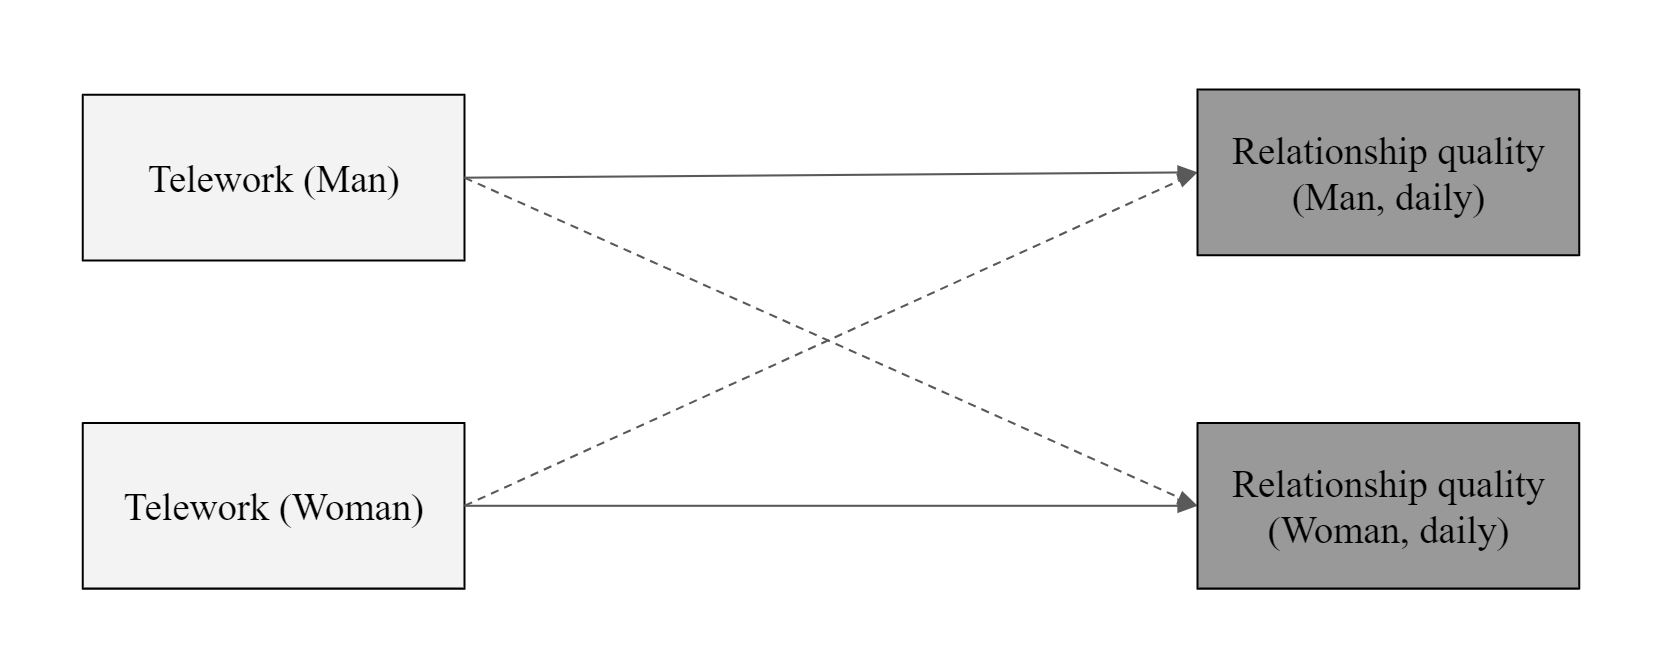
\includegraphics{C:/Users/iris_/OneDrive/Desktop/Smith/Spring 2021/PSY 364/Proj/PSY364-Yena-Iris/telework_qmi_mod.JPG}
\caption{The figure shows the model we estimated between telework mode and relationship satisfaction. We did not include the partner effect (represented in dashed lines) because the actor effect was already insignificant.}
\end{figure}

To test how telework influenced perceived chore fairness, we fit a two-intercept model with gender, the interaction term between actor's gender and actor's telework mode, and other controls such as number of children, relationship length, and actor's income (see \emph{Figure 2}).

\begin{figure}
\centering
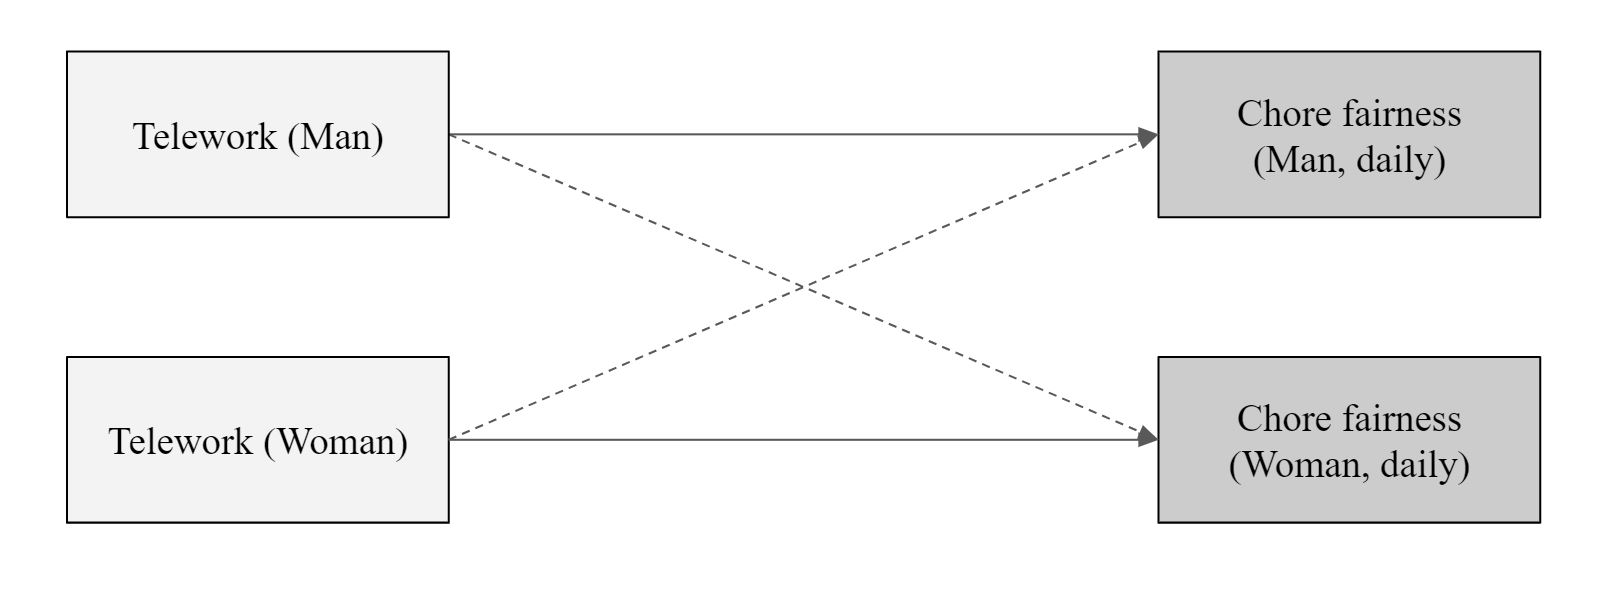
\includegraphics{C:/Users/iris_/OneDrive/Desktop/Smith/Spring 2021/PSY 364/Proj/PSY364-Yena-Iris/telework_fairness_mod.JPG}
\caption{The figure shows the model we estimated between telework mode and perceived chore fairness. We did not include the partner effect (represented in dashed lines) because the actor effect was already insignificant.}
\end{figure}

To investigate the relationship between perceived chore fairness, gender ideology, and relationship satisfaction, we first fit a simple two-intercept model, using gender, the interaction between gender and day of study, and the interaction between actor perceived chore fairness and gender to predict QMI (see \emph{Figure 3}).

\begin{figure}
\centering
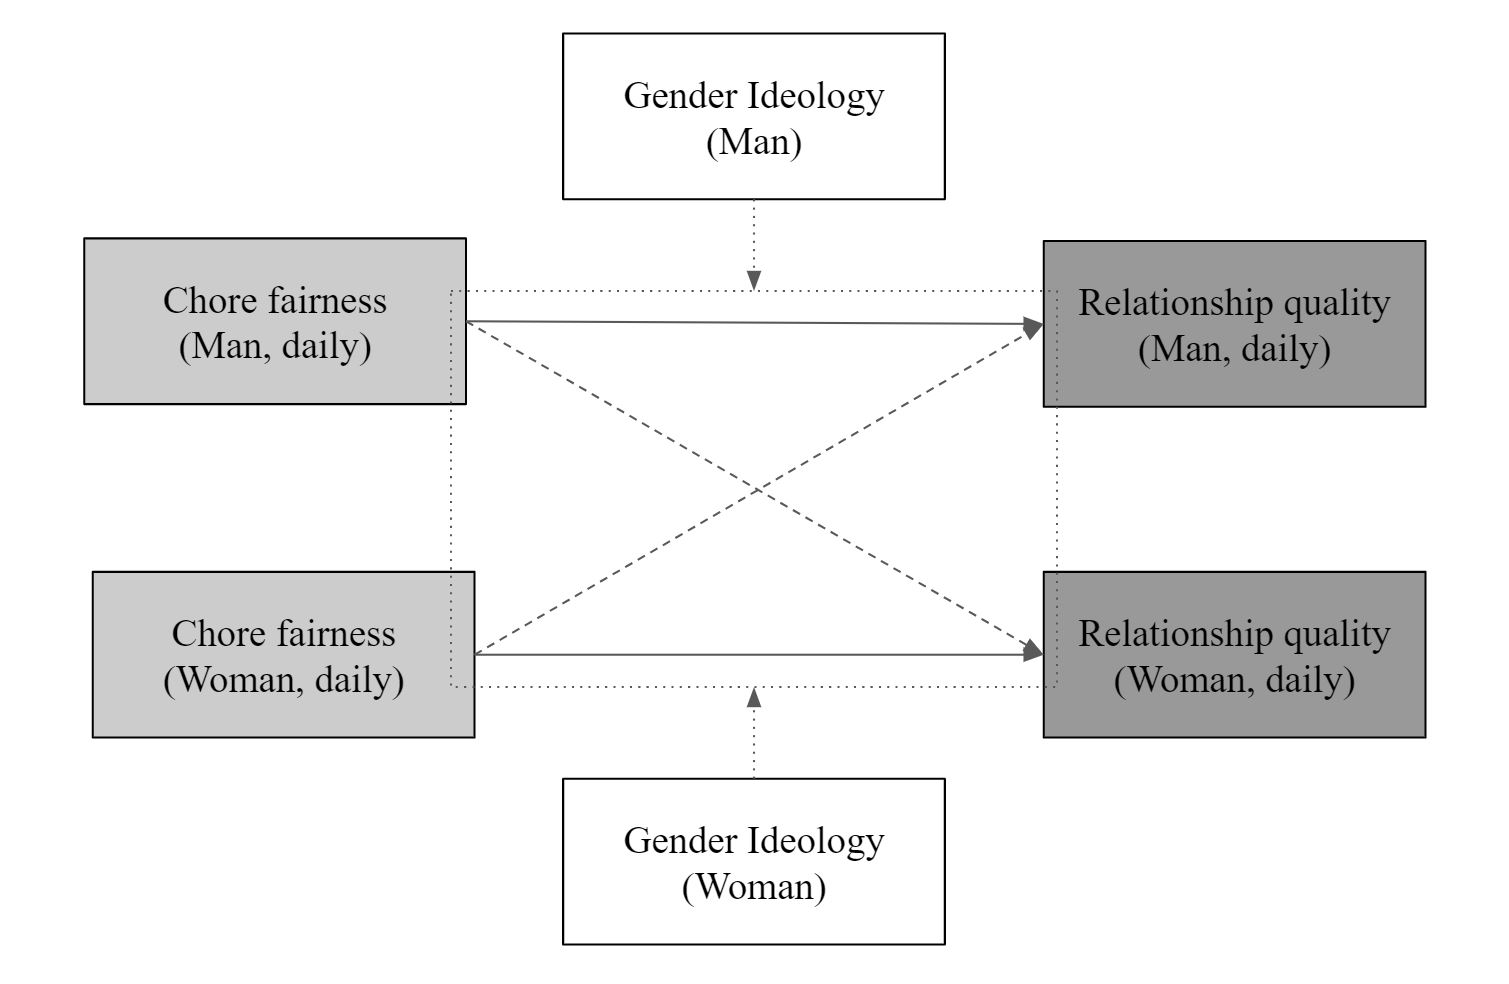
\includegraphics{C:/Users/iris_/OneDrive/Desktop/Smith/Spring 2021/PSY 364/Proj/PSY364-Yena-Iris/fairness_qmi_mod.JPG}
\caption{The figure shows the model we estimated between percieved chore fairness, gender ideology, and relationship satisfaction. The first model estimated actor effect represented by the solid lines; the second model added partner effect represented by the dashed lines; the last model added gender ideology as moderator, represented by the dotted lines.}
\end{figure}

Then, we proceeded to add a partner effect, by fitting a two-intercept model with gender, the interaction between actor's gender and day of study, the interaction between actor's perceived chore fairness and gender, the interaction between partner's perceived chore fairness and actor's gender, to predict actor's QMI (see \emph{Figure 3}).

Finally, gender ideology was added into the model as a moderator. The model included the following independent variables: gender, the interaction between actor's gender and day of study, the interaction between actor's perceived chore fairness and gender, the interaction between partner's perceived chore fairness and actor's gender, the interaction between actor's gender ideology (i.e., average gender role belief score) and actor's gender, the interaction between actor's gender ideology, actor's gender, and actor's perceived chore fairness, and the interaction between actor's gender ideology, actor's gender, and partner's perceived chore fairness, and actor's QMI was the dependent variable (see \emph{Figure 3}).

Each of the above models were estimated in two approaches -- two-intercept approach, which estimated different intercepts for men and women, and moderation approach, which produced one intercept, but also including gender as a main factor (Kenny, Kashy, \& Cook, 2020). The results reported below were from the two-intercept approach, but the moderation approach was used as well to test whether the gender difference was significant.

Each model allowed random intercepts for men and women, and for each dyad. They also accounted for the correlation between the residuals within the dyads on the same day. Lastly, different residual variances were estimated for men and women.

The scores of perceived fairness in chore division and gender ideology were centered by subtracting the original score from the grand mean, and one was subtracted from day of study, in order to make the interaction effect interpretable.

\hypertarget{main-results}{%
\subsection{Main Results}\label{main-results}}

\hypertarget{relationship-satisfaction-and-telework}{%
\subsubsection{Relationship Satisfaction and Telework}\label{relationship-satisfaction-and-telework}}

First, the actor's gender and telework mode were used to predict their own QMI score (see \emph{Table 1}). The model was relatively weak in explaining the variances in relationship satisfaction, as its pseudo-\(R^2\) was \(3.12*10^{-5}\) for men and \(3.79*10^{-5}\) for women. The intercept for men and women were 3.59 and 3.43, and gender difference was not significant (\emph{t} = -1.43, \emph{p} = 0.15). We discovered that whether the actor was teleworking did not significantly predict their own satisfaction score (men: \emph{b} = -0.082, \emph{SE} = 0.099, \emph{p} = 0.40; women: \emph{b} = 0.048, \emph{SE} = 0.10, \emph{p} = 0.65), therefore no partner effect was further investigated.

\renewcommand{\arraystretch}{0.5}
\begin{table}[!htbp] \centering 
  \caption{Relationship between telework and relationship satisfaction} 
  \label{} 
\begin{tabular}{@{\extracolsep{5pt}}lc} 
\\[-1.8ex]\hline 
\hline \\[-1.8ex] 
 & \multicolumn{1}{c}{\textit{Dependent variable:}} \\ 
\cline{2-2} 
\\[-1.8ex] & Relationship satisfaction (QMI)\\ 
\hline \\[-1.8ex] 
 Men & 3.594$^{***}$ \\ 
  & (0.089) \\ 
  & \\ 
 Women & 3.427$^{***}$ \\ 
  & (0.100) \\ 
  & \\ 
 Men * Telework & $-$0.082 \\ 
  & (0.099) \\ 
  & \\ 
 Women * Telework & 0.048 \\ 
  & (0.104) \\ 
  & \\ 
\hline \\[-1.8ex] 
Observations & 2,107 \\ 
Log Likelihood & $-$1,163.534 \\ 
Akaike Inf. Crit. & 2,347.068 \\ 
Bayesian Inf. Crit. & 2,403.579 \\ 
\hline 
\hline \\[-1.8ex] 
\textit{Note:}  & \multicolumn{1}{r}{$^{*}$p$<$0.1; $^{**}$p$<$0.05; $^{***}$p$<$0.01} \\ 
\end{tabular} 
\end{table}

\hypertarget{perceived-chore-fairness-and-telework}{%
\subsubsection{Perceived Chore Fairness and Telework}\label{perceived-chore-fairness-and-telework}}

Next, we predicted actor's perceived chore fairness with their gender, telework mode, number of children, their relationship in years, and income (see \emph{Table 2}). The model's total explanatory power was weak because pseudo-\(R^2\) was 0.032 for men and 0.011 for women. According to the results, the intercept for men was 0.29 and the intercept for women was 0.35, but the difference of intercept between men and women was not significant (\emph{t} = 0.19, \emph{p} = 0.85). Whether the individual was teleworking or not was not a significant predictor of relationship satisfaction (men: \emph{b} = -0.07, \emph{SE} = 0.19, \emph{p} = 0.71; women: \emph{b} = -0.29, \emph{SE} = 0.26, \emph{p} = 0.26).

The control variables did not have a significant effect on perceived chore fairness either. The coefficient for the number of children was 0.014, yet it was not significant (\emph{SE} = 0.084, \emph{p} = 0.87). Similarly, the relationship length and income did not significantly predict perceived chore fairness either (relationship length: \emph{b} = -0.012, \emph{SE} = 0.0081, \emph{p} = 0.14).

Since the actor effect of teleworking was already insignificant, we did not continue testing the partner effect of teleworking on perceived chore fairness.

\begin{table}[!htbp] \centering 
  \caption{Relationship between telework and perceived chore fairness} 
  \label{} 
\begin{tabular}{@{\extracolsep{5pt}}lc} 
\\[-1.8ex]\hline 
\hline \\[-1.8ex] 
 & \multicolumn{1}{c}{\textit{Dependent variable:}} \\ 
\cline{2-2} 
\\[-1.8ex] & Perceived chore fairness \\ 
\hline \\[-1.8ex] 
 Men & 0.294 \\ 
  & (0.236) \\ 
  & \\ 
 Women & 0.346 \\ 
  & (0.306) \\ 
  & \\ 
 Number of children & 0.014 \\ 
  & (0.084) \\ 
  & \\ 
 Relationship length & $-$0.012 \\ 
  & (0.008) \\ 
  & \\ 
 Income & 0.00000 \\ 
  & (0.00000) \\ 
  & \\ 
 Men * Telework & $-$0.071 \\ 
  & (0.189) \\ 
  & \\ 
 Women * Telework & $-$0.289 \\ 
  & (0.257) \\ 
  & \\ 
\hline \\[-1.8ex] 
Observations & 1,807 \\ 
Log Likelihood & $-$1,846.967 \\ 
Akaike Inf. Crit. & 3,719.933 \\ 
Bayesian Inf. Crit. & 3,791.375 \\ 
\hline 
\hline \\[-1.8ex] 
\textit{Note:}  & \multicolumn{1}{r}{$^{*}$p$<$0.1; $^{**}$p$<$0.05; $^{***}$p$<$0.01} \\
\end{tabular} 
\end{table}

\hypertarget{relationship-satisfaction-perceived-chore-fairness-and-gender-ideology}{%
\subsubsection{Relationship Satisfaction, Perceived Chore Fairness and Gender Ideology}\label{relationship-satisfaction-perceived-chore-fairness-and-gender-ideology}}

\begin{figure}
\centering
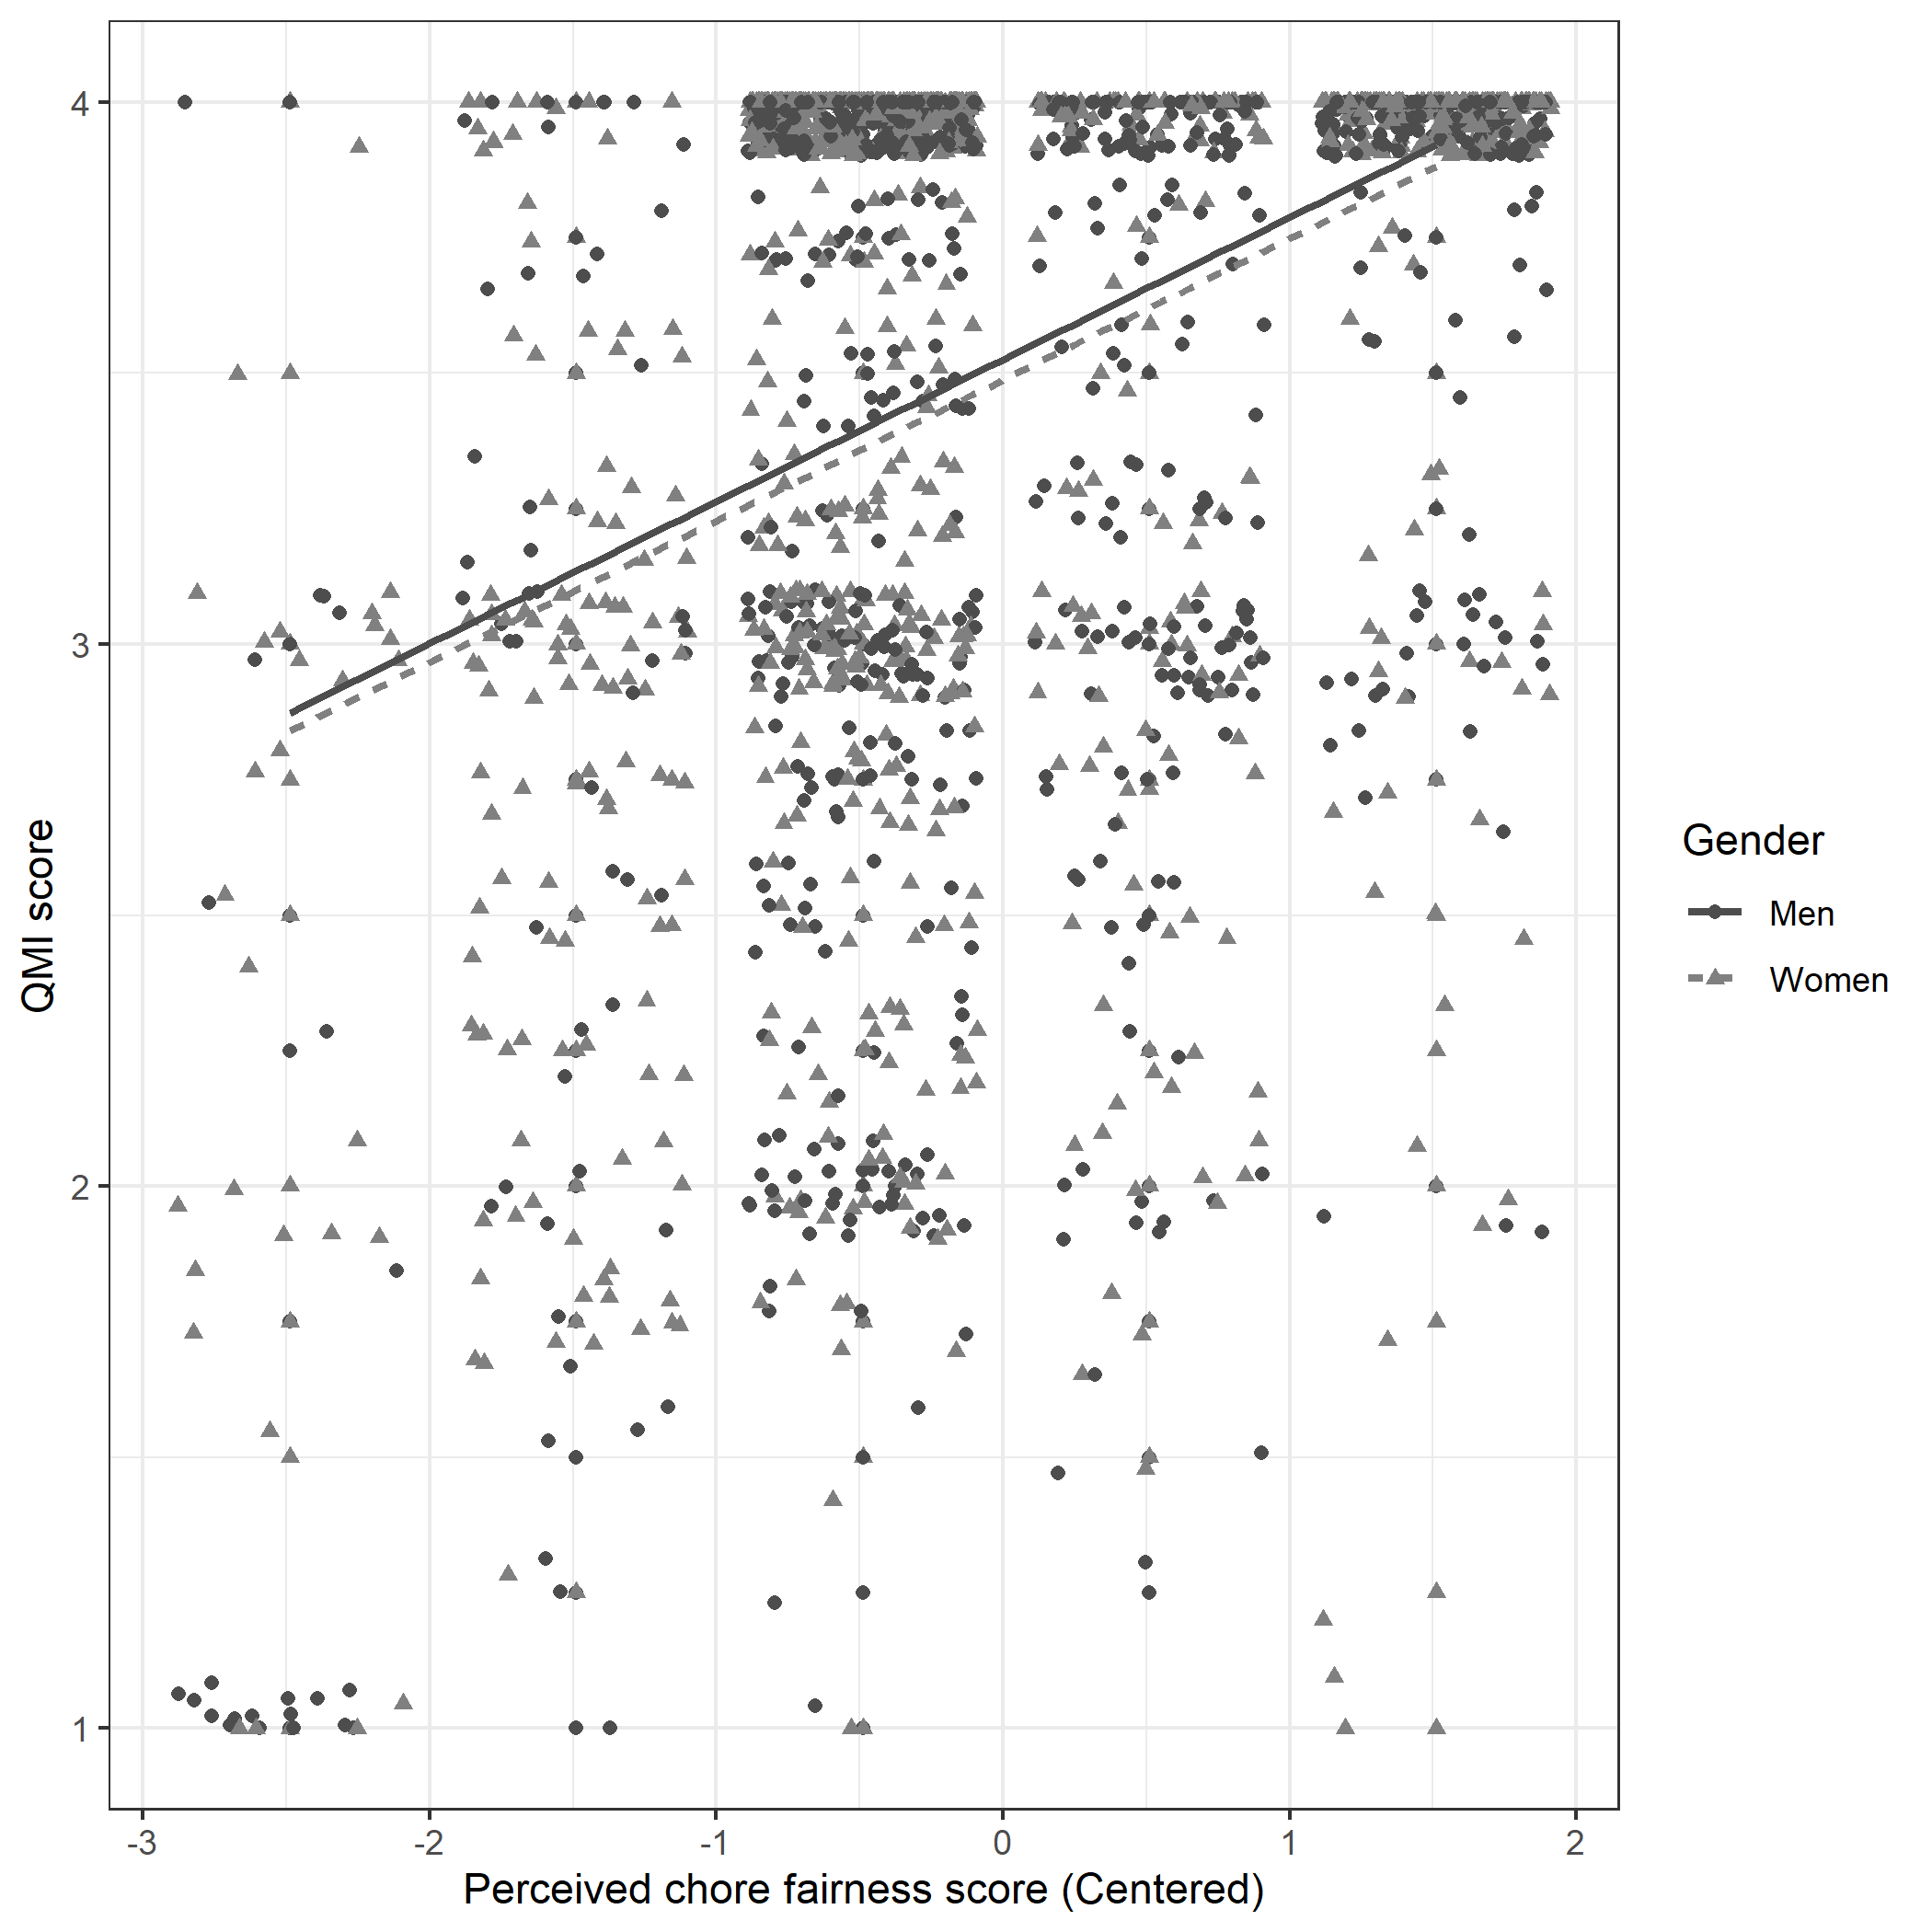
\includegraphics{C:/Users/iris_/OneDrive/Desktop/Smith/Spring 2021/PSY 364/Proj/PSY364-Yena-Iris/qmi_fairness.png}
\caption{The figure shows that perceived chore fairness is positively correlated with satisfaction. Women in general reported lower satisfaction than men.}
\end{figure}

To investigate the relationship between relationship satisfaction and chore fairness, a two-intercept multilevel model without accounting for partner effect was first estimated (see \emph{Table 3}). The results showed that the intercepts for men and women were 3.56 and 3.43 respectively, and according to the moderation approach model, women's intercept was significantly lower than men (\emph{SE} = 0.050, \emph{p} = 0.0059) (see \emph{Figure 4}). The interaction term between gender and day of study demonstrated that for men, their satisfaction score was not significantly predicted by day of study (\emph{b} = -0.0029, \emph{SE} = 0.0027, \emph{p} = 0.29), but day of study was a significant positive predictor for women's satisfaction score (\emph{b} = 0.0066, \emph{SE} = 0.0031, \emph{p} = 0.036). In addition, perceived chore fairness score significantly positively predicted both male and female's QMI for a given day (see \emph{Figure 4}), and the coefficient for women was higher than that for men, indicating that a one point increase in perceived chore fairness score could led to a higher increase in satisfaction score for women than for men (men: \emph{b} = 0.069, \emph{SE} = 0.018, \emph{p} = 0.0001; women: \emph{b} = 0.085, \emph{SE} = 0.019, \emph{p} = 0.0000). The pseudo-\(R^2\) in this model was 0.0065 for women, and 0.0063 for men.

We continued testing the relationship between perceived chore fairness and QMI with partner effect added (see \emph{Table 3}). The associations found in the previous model were retained. Partner's perceived fairness in chore division was negatively correlated with actor's satisfaction for both women and men, implying that the less unfair the partner perceived for their own chore, the lower satisfaction the actor felt, but the effect was insignificant for either men (\emph{b} = -0.0083, \emph{SE} = 0.018, \emph{p} = 0.65) or women (\emph{b} = -0.0034, \emph{SE} = 0.021, \emph{p} = 0.87). The pseudo-\(R^2\) in this model was 0.0059 for women, and 0.0057 for men.

The effect of gender ideology was further incorporated into the model (see \emph{Table 3}). First, a positive association was found between centered gender role belief score and relationship satisfaction for both gender, meaning that the model would predict an individual holding a more traditional gender ideology to have a higher relationship satisfaction score. However, the relationship was not statistically significant (men: \emph{b} = 0.072, \emph{SE} = 0.082, \emph{p} = 0.38; women: \emph{b} = 0.043, \emph{SE} = 0.073, \emph{p} = 0.56). To test whether gender ideology was a moderator, we also included the interaction between actor's gender, actor's gender ideology, and actor's perceived chore fairness, yet the term was not significant for both men (\emph{b} = -0.036, \emph{SE} = 0.025, \emph{p} = 0.16) and women (\emph{b} = -0.036, \emph{SE} = 0.030, \emph{p} = 0.23). The interaction between actor's gender, actor's gender ideology, and partner's perceived chore fairness did not significantly predict actor's relationship satisfaction either (men: \emph{b} = 0.00059, \emph{SE} = 0.028, \emph{p} = 0.98; women: \emph{b} = -0.016, \emph{SE} = 0.029, \emph{p} = 0.58). The model's pseudo-\(R^2\) was 0.0048 for men and 0.0045 for women, which demonstrated that it did not account for much variance compared to an empty model with no explanatory variables.\footnote{The more complicated models had even lower \(R^2\); is something wrong here?}

\begin{Shaded}
\begin{Highlighting}[]
\KeywordTok{library}\NormalTok{(broom.mixed)}
\end{Highlighting}
\end{Shaded}

\begin{verbatim}
## Warning: package 'broom.mixed' was built under R version 4.0.5
\end{verbatim}

\begin{verbatim}
## Warning in checkMatrixPackageVersion(): Package version inconsistency detected.
## TMB was built with Matrix version 1.3.2
## Current Matrix version is 1.2.18
## Please re-install 'TMB' from source using install.packages('TMB', type = 'source') or ask CRAN for a binary version of 'TMB' matching CRAN's 'Matrix' package
\end{verbatim}

\begin{Shaded}
\begin{Highlighting}[]
\NormalTok{huxtable}\OperatorTok{::}\KeywordTok{to\_latex}\NormalTok{(huxtable}\OperatorTok{::}\KeywordTok{huxreg}\NormalTok{(}\KeywordTok{list}\NormalTok{(}
                 \StringTok{"Model 1"}\NormalTok{ =}\StringTok{ }\NormalTok{mod\_qmi\_chore\_}\DecValTok{1}\NormalTok{, }
                 \StringTok{"Model 2"}\NormalTok{ =}\StringTok{ }\NormalTok{mod\_qmi\_chore\_}\DecValTok{2}\NormalTok{,}
                 \StringTok{"Model 3"}\NormalTok{ =}\StringTok{ }\NormalTok{mod\_qmi\_chore\_}\DecValTok{2}\NormalTok{)))}
\end{Highlighting}
\end{Shaded}

\begin{verbatim}
## Warning in huxtable::huxreg(list(`Model 1` = mod_qmi_chore_1, `Model 2` = mod_qmi_chore_2, : Unrecognized statistics: r.squared
## Try setting `statistics` explicitly in the call to `huxreg()`
\end{verbatim}

{[}1{]} ``\n\n\texttt{\{=latex\}\textbackslash{}n\ \textbackslash{}n\ \ \textbackslash{}\textbackslash{}providecommand\{\textbackslash{}\textbackslash{}huxb\}{[}2{]}\{\textbackslash{}\textbackslash{}arrayrulecolor{[}RGB{]}\{\#1\}\textbackslash{}\textbackslash{}global\textbackslash{}\textbackslash{}arrayrulewidth=\#2pt\}\textbackslash{}n\ \ \textbackslash{}\textbackslash{}providecommand\{\textbackslash{}\textbackslash{}huxvb\}{[}2{]}\{\textbackslash{}\textbackslash{}color{[}RGB{]}\{\#1\}\textbackslash{}\textbackslash{}vrule\ width\ \#2pt\}\textbackslash{}n\ \ \textbackslash{}\textbackslash{}providecommand\{\textbackslash{}\textbackslash{}huxtpad\}{[}1{]}\{\textbackslash{}\textbackslash{}rule\{0pt\}\{\#1\}\}\textbackslash{}n\ \ \textbackslash{}\textbackslash{}providecommand\{\textbackslash{}\textbackslash{}huxbpad\}{[}1{]}\{\textbackslash{}\textbackslash{}rule{[}-\#1{]}\{0pt\}\{\#1\}\}\textbackslash{}n\textbackslash{}n\textbackslash{}\textbackslash{}begin\{table\}{[}ht{]}\textbackslash{}n\textbackslash{}\textbackslash{}begin\{centerbox\}\textbackslash{}n\textbackslash{}\textbackslash{}begin\{threeparttable\}\textbackslash{}n\ \textbackslash{}\textbackslash{}label\{tab:unnamed-chunk-4\}\textbackslash{}n\textbackslash{}\textbackslash{}setlength\{\textbackslash{}\textbackslash{}tabcolsep\}\{0pt\}\textbackslash{}n\textbackslash{}\textbackslash{}begin\{tabular\}\{l\ l\ l\ l\}\textbackslash{}n\textbackslash{}n\textbackslash{}n\textbackslash{}\textbackslash{}hhline\{\textgreater{}\{\textbackslash{}\textbackslash{}huxb\{0,\ 0,\ 0\}\{0.8\}\}-\textgreater{}\{\textbackslash{}\textbackslash{}huxb\{0,\ 0,\ 0\}\{0.8\}\}-\textgreater{}\{\textbackslash{}\textbackslash{}huxb\{0,\ 0,\ 0\}\{0.8\}\}-\textgreater{}\{\textbackslash{}\textbackslash{}huxb\{0,\ 0,\ 0\}\{0.8\}\}-\}\textbackslash{}n\textbackslash{}\textbackslash{}arrayrulecolor\{black\}\textbackslash{}n\textbackslash{}n\textbackslash{}\textbackslash{}multicolumn\{1\}\{!\{\textbackslash{}\textbackslash{}huxvb\{0,\ 0,\ 0\}\{0\}\}c!\{\textbackslash{}\textbackslash{}huxvb\{0,\ 0,\ 0\}\{0\}\}\}\{\textbackslash{}\textbackslash{}huxtpad\{6pt\ +\ 1em\}\textbackslash{}\textbackslash{}centering\ \textbackslash{}\textbackslash{}hspace\{6pt\}\ \ \textbackslash{}\textbackslash{}hspace\{6pt\}\textbackslash{}\textbackslash{}huxbpad\{6pt\}\}\ \&\textbackslash{}n\textbackslash{}\textbackslash{}multicolumn\{1\}\{c!\{\textbackslash{}\textbackslash{}huxvb\{0,\ 0,\ 0\}\{0\}\}\}\{\textbackslash{}\textbackslash{}huxtpad\{6pt\ +\ 1em\}\textbackslash{}\textbackslash{}centering\ \textbackslash{}\textbackslash{}hspace\{6pt\}\ Model\ 1\ \textbackslash{}\textbackslash{}hspace\{6pt\}\textbackslash{}\textbackslash{}huxbpad\{6pt\}\}\ \&\textbackslash{}n\textbackslash{}\textbackslash{}multicolumn\{1\}\{c!\{\textbackslash{}\textbackslash{}huxvb\{0,\ 0,\ 0\}\{0\}\}\}\{\textbackslash{}\textbackslash{}huxtpad\{6pt\ +\ 1em\}\textbackslash{}\textbackslash{}centering\ \textbackslash{}\textbackslash{}hspace\{6pt\}\ Model\ 2\ \textbackslash{}\textbackslash{}hspace\{6pt\}\textbackslash{}\textbackslash{}huxbpad\{6pt\}\}\ \&\textbackslash{}n\textbackslash{}\textbackslash{}multicolumn\{1\}\{c!\{\textbackslash{}\textbackslash{}huxvb\{0,\ 0,\ 0\}\{0\}\}\}\{\textbackslash{}\textbackslash{}huxtpad\{6pt\ +\ 1em\}\textbackslash{}\textbackslash{}centering\ \textbackslash{}\textbackslash{}hspace\{6pt\}\ Model\ 3\ \textbackslash{}\textbackslash{}hspace\{6pt\}\textbackslash{}\textbackslash{}huxbpad\{6pt\}\}\ \textbackslash{}\textbackslash{}tabularnewline{[}-0.5pt{]}\textbackslash{}n\textbackslash{}n\textbackslash{}n\textbackslash{}\textbackslash{}hhline\{\textgreater{}\{\textbackslash{}\textbackslash{}huxb\{255,\ 255,\ 255\}\{0.4\}\}-\textgreater{}\{\textbackslash{}\textbackslash{}huxb\{0,\ 0,\ 0\}\{0.4\}\}-\textgreater{}\{\textbackslash{}\textbackslash{}huxb\{0,\ 0,\ 0\}\{0.4\}\}-\textgreater{}\{\textbackslash{}\textbackslash{}huxb\{0,\ 0,\ 0\}\{0.4\}\}-\}\textbackslash{}n\textbackslash{}\textbackslash{}arrayrulecolor\{black\}\textbackslash{}n\textbackslash{}n\textbackslash{}\textbackslash{}multicolumn\{1\}\{!\{\textbackslash{}\textbackslash{}huxvb\{0,\ 0,\ 0\}\{0\}\}l!\{\textbackslash{}\textbackslash{}huxvb\{0,\ 0,\ 0\}\{0\}\}\}\{\textbackslash{}\textbackslash{}huxtpad\{6pt\ +\ 1em\}\textbackslash{}\textbackslash{}raggedright\ \textbackslash{}\textbackslash{}hspace\{6pt\}\ gender\textbackslash{}\textbackslash{}\_chr\textbackslash{}\textbackslash{}\_AM\ \textbackslash{}\textbackslash{}hspace\{6pt\}\textbackslash{}\textbackslash{}huxbpad\{6pt\}\}\ \&\textbackslash{}n\textbackslash{}\textbackslash{}multicolumn\{1\}\{r!\{\textbackslash{}\textbackslash{}huxvb\{0,\ 0,\ 0\}\{0\}\}\}\{\textbackslash{}\textbackslash{}huxtpad\{6pt\ +\ 1em\}\textbackslash{}\textbackslash{}raggedleft\ \textbackslash{}\textbackslash{}hspace\{6pt\}\ 3.563\ ***\ \textbackslash{}\textbackslash{}hspace\{6pt\}\textbackslash{}\textbackslash{}huxbpad\{6pt\}\}\ \&\textbackslash{}n\textbackslash{}\textbackslash{}multicolumn\{1\}\{r!\{\textbackslash{}\textbackslash{}huxvb\{0,\ 0,\ 0\}\{0\}\}\}\{\textbackslash{}\textbackslash{}huxtpad\{6pt\ +\ 1em\}\textbackslash{}\textbackslash{}raggedleft\ \textbackslash{}\textbackslash{}hspace\{6pt\}\ 3.563\ ***\ \textbackslash{}\textbackslash{}hspace\{6pt\}\textbackslash{}\textbackslash{}huxbpad\{6pt\}\}\ \&\textbackslash{}n\textbackslash{}\textbackslash{}multicolumn\{1\}\{r!\{\textbackslash{}\textbackslash{}huxvb\{0,\ 0,\ 0\}\{0\}\}\}\{\textbackslash{}\textbackslash{}huxtpad\{6pt\ +\ 1em\}\textbackslash{}\textbackslash{}raggedleft\ \textbackslash{}\textbackslash{}hspace\{6pt\}\ 3.563\ ***\ \textbackslash{}\textbackslash{}hspace\{6pt\}\textbackslash{}\textbackslash{}huxbpad\{6pt\}\}\ \textbackslash{}\textbackslash{}tabularnewline{[}-0.5pt{]}\textbackslash{}n\textbackslash{}n\textbackslash{}n\textbackslash{}\textbackslash{}hhline\{\}\textbackslash{}n\textbackslash{}\textbackslash{}arrayrulecolor\{black\}\textbackslash{}n\textbackslash{}n\textbackslash{}\textbackslash{}multicolumn\{1\}\{!\{\textbackslash{}\textbackslash{}huxvb\{0,\ 0,\ 0\}\{0\}\}l!\{\textbackslash{}\textbackslash{}huxvb\{0,\ 0,\ 0\}\{0\}\}\}\{\textbackslash{}\textbackslash{}huxtpad\{6pt\ +\ 1em\}\textbackslash{}\textbackslash{}raggedright\ \textbackslash{}\textbackslash{}hspace\{6pt\}\ \ \textbackslash{}\textbackslash{}hspace\{6pt\}\textbackslash{}\textbackslash{}huxbpad\{6pt\}\}\ \&\textbackslash{}n\textbackslash{}\textbackslash{}multicolumn\{1\}\{r!\{\textbackslash{}\textbackslash{}huxvb\{0,\ 0,\ 0\}\{0\}\}\}\{\textbackslash{}\textbackslash{}huxtpad\{6pt\ +\ 1em\}\textbackslash{}\textbackslash{}raggedleft\ \textbackslash{}\textbackslash{}hspace\{6pt\}\ (0.070)\textasciitilde{}\textasciitilde{}\textasciitilde{}\ \textbackslash{}\textbackslash{}hspace\{6pt\}\textbackslash{}\textbackslash{}huxbpad\{6pt\}\}\ \&\textbackslash{}n\textbackslash{}\textbackslash{}multicolumn\{1\}\{r!\{\textbackslash{}\textbackslash{}huxvb\{0,\ 0,\ 0\}\{0\}\}\}\{\textbackslash{}\textbackslash{}huxtpad\{6pt\ +\ 1em\}\textbackslash{}\textbackslash{}raggedleft\ \textbackslash{}\textbackslash{}hspace\{6pt\}\ (0.070)\textasciitilde{}\textasciitilde{}\textasciitilde{}\ \textbackslash{}\textbackslash{}hspace\{6pt\}\textbackslash{}\textbackslash{}huxbpad\{6pt\}\}\ \&\textbackslash{}n\textbackslash{}\textbackslash{}multicolumn\{1\}\{r!\{\textbackslash{}\textbackslash{}huxvb\{0,\ 0,\ 0\}\{0\}\}\}\{\textbackslash{}\textbackslash{}huxtpad\{6pt\ +\ 1em\}\textbackslash{}\textbackslash{}raggedleft\ \textbackslash{}\textbackslash{}hspace\{6pt\}\ (0.070)\textasciitilde{}\textasciitilde{}\textasciitilde{}\ \textbackslash{}\textbackslash{}hspace\{6pt\}\textbackslash{}\textbackslash{}huxbpad\{6pt\}\}\ \textbackslash{}\textbackslash{}tabularnewline{[}-0.5pt{]}\textbackslash{}n\textbackslash{}n\textbackslash{}n\textbackslash{}\textbackslash{}hhline\{\}\textbackslash{}n\textbackslash{}\textbackslash{}arrayrulecolor\{black\}\textbackslash{}n\textbackslash{}n\textbackslash{}\textbackslash{}multicolumn\{1\}\{!\{\textbackslash{}\textbackslash{}huxvb\{0,\ 0,\ 0\}\{0\}\}l!\{\textbackslash{}\textbackslash{}huxvb\{0,\ 0,\ 0\}\{0\}\}\}\{\textbackslash{}\textbackslash{}huxtpad\{6pt\ +\ 1em\}\textbackslash{}\textbackslash{}raggedright\ \textbackslash{}\textbackslash{}hspace\{6pt\}\ gender\textbackslash{}\textbackslash{}\_chr\textbackslash{}\textbackslash{}\_AW\ \textbackslash{}\textbackslash{}hspace\{6pt\}\textbackslash{}\textbackslash{}huxbpad\{6pt\}\}\ \&\textbackslash{}n\textbackslash{}\textbackslash{}multicolumn\{1\}\{r!\{\textbackslash{}\textbackslash{}huxvb\{0,\ 0,\ 0\}\{0\}\}\}\{\textbackslash{}\textbackslash{}huxtpad\{6pt\ +\ 1em\}\textbackslash{}\textbackslash{}raggedleft\ \textbackslash{}\textbackslash{}hspace\{6pt\}\ 3.426\ ***\ \textbackslash{}\textbackslash{}hspace\{6pt\}\textbackslash{}\textbackslash{}huxbpad\{6pt\}\}\ \&\textbackslash{}n\textbackslash{}\textbackslash{}multicolumn\{1\}\{r!\{\textbackslash{}\textbackslash{}huxvb\{0,\ 0,\ 0\}\{0\}\}\}\{\textbackslash{}\textbackslash{}huxtpad\{6pt\ +\ 1em\}\textbackslash{}\textbackslash{}raggedleft\ \textbackslash{}\textbackslash{}hspace\{6pt\}\ 3.426\ ***\ \textbackslash{}\textbackslash{}hspace\{6pt\}\textbackslash{}\textbackslash{}huxbpad\{6pt\}\}\ \&\textbackslash{}n\textbackslash{}\textbackslash{}multicolumn\{1\}\{r!\{\textbackslash{}\textbackslash{}huxvb\{0,\ 0,\ 0\}\{0\}\}\}\{\textbackslash{}\textbackslash{}huxtpad\{6pt\ +\ 1em\}\textbackslash{}\textbackslash{}raggedleft\ \textbackslash{}\textbackslash{}hspace\{6pt\}\ 3.426\ ***\ \textbackslash{}\textbackslash{}hspace\{6pt\}\textbackslash{}\textbackslash{}huxbpad\{6pt\}\}\ \textbackslash{}\textbackslash{}tabularnewline{[}-0.5pt{]}\textbackslash{}n\textbackslash{}n\textbackslash{}n\textbackslash{}\textbackslash{}hhline\{\}\textbackslash{}n\textbackslash{}\textbackslash{}arrayrulecolor\{black\}\textbackslash{}n\textbackslash{}n\textbackslash{}\textbackslash{}multicolumn\{1\}\{!\{\textbackslash{}\textbackslash{}huxvb\{0,\ 0,\ 0\}\{0\}\}l!\{\textbackslash{}\textbackslash{}huxvb\{0,\ 0,\ 0\}\{0\}\}\}\{\textbackslash{}\textbackslash{}huxtpad\{6pt\ +\ 1em\}\textbackslash{}\textbackslash{}raggedright\ \textbackslash{}\textbackslash{}hspace\{6pt\}\ \ \textbackslash{}\textbackslash{}hspace\{6pt\}\textbackslash{}\textbackslash{}huxbpad\{6pt\}\}\ \&\textbackslash{}n\textbackslash{}\textbackslash{}multicolumn\{1\}\{r!\{\textbackslash{}\textbackslash{}huxvb\{0,\ 0,\ 0\}\{0\}\}\}\{\textbackslash{}\textbackslash{}huxtpad\{6pt\ +\ 1em\}\textbackslash{}\textbackslash{}raggedleft\ \textbackslash{}\textbackslash{}hspace\{6pt\}\ (0.066)\textasciitilde{}\textasciitilde{}\textasciitilde{}\ \textbackslash{}\textbackslash{}hspace\{6pt\}\textbackslash{}\textbackslash{}huxbpad\{6pt\}\}\ \&\textbackslash{}n\textbackslash{}\textbackslash{}multicolumn\{1\}\{r!\{\textbackslash{}\textbackslash{}huxvb\{0,\ 0,\ 0\}\{0\}\}\}\{\textbackslash{}\textbackslash{}huxtpad\{6pt\ +\ 1em\}\textbackslash{}\textbackslash{}raggedleft\ \textbackslash{}\textbackslash{}hspace\{6pt\}\ (0.067)\textasciitilde{}\textasciitilde{}\textasciitilde{}\ \textbackslash{}\textbackslash{}hspace\{6pt\}\textbackslash{}\textbackslash{}huxbpad\{6pt\}\}\ \&\textbackslash{}n\textbackslash{}\textbackslash{}multicolumn\{1\}\{r!\{\textbackslash{}\textbackslash{}huxvb\{0,\ 0,\ 0\}\{0\}\}\}\{\textbackslash{}\textbackslash{}huxtpad\{6pt\ +\ 1em\}\textbackslash{}\textbackslash{}raggedleft\ \textbackslash{}\textbackslash{}hspace\{6pt\}\ (0.067)\textasciitilde{}\textasciitilde{}\textasciitilde{}\ \textbackslash{}\textbackslash{}hspace\{6pt\}\textbackslash{}\textbackslash{}huxbpad\{6pt\}\}\ \textbackslash{}\textbackslash{}tabularnewline{[}-0.5pt{]}\textbackslash{}n\textbackslash{}n\textbackslash{}n\textbackslash{}\textbackslash{}hhline\{\}\textbackslash{}n\textbackslash{}\textbackslash{}arrayrulecolor\{black\}\textbackslash{}n\textbackslash{}n\textbackslash{}\textbackslash{}multicolumn\{1\}\{!\{\textbackslash{}\textbackslash{}huxvb\{0,\ 0,\ 0\}\{0\}\}l!\{\textbackslash{}\textbackslash{}huxvb\{0,\ 0,\ 0\}\{0\}\}\}\{\textbackslash{}\textbackslash{}huxtpad\{6pt\ +\ 1em\}\textbackslash{}\textbackslash{}raggedright\ \textbackslash{}\textbackslash{}hspace\{6pt\}\ gender\textbackslash{}\textbackslash{}\_chr\textbackslash{}\textbackslash{}\_AM:day\textbackslash{}\textbackslash{}\_of\textbackslash{}\textbackslash{}\_study\textbackslash{}\textbackslash{}\_A\ \textbackslash{}\textbackslash{}hspace\{6pt\}\textbackslash{}\textbackslash{}huxbpad\{6pt\}\}\ \&\textbackslash{}n\textbackslash{}\textbackslash{}multicolumn\{1\}\{r!\{\textbackslash{}\textbackslash{}huxvb\{0,\ 0,\ 0\}\{0\}\}\}\{\textbackslash{}\textbackslash{}huxtpad\{6pt\ +\ 1em\}\textbackslash{}\textbackslash{}raggedleft\ \textbackslash{}\textbackslash{}hspace\{6pt\}\ -0.003\textasciitilde{}\textasciitilde{}\textasciitilde{}\textasciitilde{}\ \textbackslash{}\textbackslash{}hspace\{6pt\}\textbackslash{}\textbackslash{}huxbpad\{6pt\}\}\ \&\textbackslash{}n\textbackslash{}\textbackslash{}multicolumn\{1\}\{r!\{\textbackslash{}\textbackslash{}huxvb\{0,\ 0,\ 0\}\{0\}\}\}\{\textbackslash{}\textbackslash{}huxtpad\{6pt\ +\ 1em\}\textbackslash{}\textbackslash{}raggedleft\ \textbackslash{}\textbackslash{}hspace\{6pt\}\ -0.003\textasciitilde{}\textasciitilde{}\textasciitilde{}\textasciitilde{}\ \textbackslash{}\textbackslash{}hspace\{6pt\}\textbackslash{}\textbackslash{}huxbpad\{6pt\}\}\ \&\textbackslash{}n\textbackslash{}\textbackslash{}multicolumn\{1\}\{r!\{\textbackslash{}\textbackslash{}huxvb\{0,\ 0,\ 0\}\{0\}\}\}\{\textbackslash{}\textbackslash{}huxtpad\{6pt\ +\ 1em\}\textbackslash{}\textbackslash{}raggedleft\ \textbackslash{}\textbackslash{}hspace\{6pt\}\ -0.003\textasciitilde{}\textasciitilde{}\textasciitilde{}\textasciitilde{}\ \textbackslash{}\textbackslash{}hspace\{6pt\}\textbackslash{}\textbackslash{}huxbpad\{6pt\}\}\ \textbackslash{}\textbackslash{}tabularnewline{[}-0.5pt{]}\textbackslash{}n\textbackslash{}n\textbackslash{}n\textbackslash{}\textbackslash{}hhline\{\}\textbackslash{}n\textbackslash{}\textbackslash{}arrayrulecolor\{black\}\textbackslash{}n\textbackslash{}n\textbackslash{}\textbackslash{}multicolumn\{1\}\{!\{\textbackslash{}\textbackslash{}huxvb\{0,\ 0,\ 0\}\{0\}\}l!\{\textbackslash{}\textbackslash{}huxvb\{0,\ 0,\ 0\}\{0\}\}\}\{\textbackslash{}\textbackslash{}huxtpad\{6pt\ +\ 1em\}\textbackslash{}\textbackslash{}raggedright\ \textbackslash{}\textbackslash{}hspace\{6pt\}\ \ \textbackslash{}\textbackslash{}hspace\{6pt\}\textbackslash{}\textbackslash{}huxbpad\{6pt\}\}\ \&\textbackslash{}n\textbackslash{}\textbackslash{}multicolumn\{1\}\{r!\{\textbackslash{}\textbackslash{}huxvb\{0,\ 0,\ 0\}\{0\}\}\}\{\textbackslash{}\textbackslash{}huxtpad\{6pt\ +\ 1em\}\textbackslash{}\textbackslash{}raggedleft\ \textbackslash{}\textbackslash{}hspace\{6pt\}\ (0.003)\textasciitilde{}\textasciitilde{}\textasciitilde{}\ \textbackslash{}\textbackslash{}hspace\{6pt\}\textbackslash{}\textbackslash{}huxbpad\{6pt\}\}\ \&\textbackslash{}n\textbackslash{}\textbackslash{}multicolumn\{1\}\{r!\{\textbackslash{}\textbackslash{}huxvb\{0,\ 0,\ 0\}\{0\}\}\}\{\textbackslash{}\textbackslash{}huxtpad\{6pt\ +\ 1em\}\textbackslash{}\textbackslash{}raggedleft\ \textbackslash{}\textbackslash{}hspace\{6pt\}\ (0.003)\textasciitilde{}\textasciitilde{}\textasciitilde{}\ \textbackslash{}\textbackslash{}hspace\{6pt\}\textbackslash{}\textbackslash{}huxbpad\{6pt\}\}\ \&\textbackslash{}n\textbackslash{}\textbackslash{}multicolumn\{1\}\{r!\{\textbackslash{}\textbackslash{}huxvb\{0,\ 0,\ 0\}\{0\}\}\}\{\textbackslash{}\textbackslash{}huxtpad\{6pt\ +\ 1em\}\textbackslash{}\textbackslash{}raggedleft\ \textbackslash{}\textbackslash{}hspace\{6pt\}\ (0.003)\textasciitilde{}\textasciitilde{}\textasciitilde{}\ \textbackslash{}\textbackslash{}hspace\{6pt\}\textbackslash{}\textbackslash{}huxbpad\{6pt\}\}\ \textbackslash{}\textbackslash{}tabularnewline{[}-0.5pt{]}\textbackslash{}n\textbackslash{}n\textbackslash{}n\textbackslash{}\textbackslash{}hhline\{\}\textbackslash{}n\textbackslash{}\textbackslash{}arrayrulecolor\{black\}\textbackslash{}n\textbackslash{}n\textbackslash{}\textbackslash{}multicolumn\{1\}\{!\{\textbackslash{}\textbackslash{}huxvb\{0,\ 0,\ 0\}\{0\}\}l!\{\textbackslash{}\textbackslash{}huxvb\{0,\ 0,\ 0\}\{0\}\}\}\{\textbackslash{}\textbackslash{}huxtpad\{6pt\ +\ 1em\}\textbackslash{}\textbackslash{}raggedright\ \textbackslash{}\textbackslash{}hspace\{6pt\}\ gender\textbackslash{}\textbackslash{}\_chr\textbackslash{}\textbackslash{}\_AW:day\textbackslash{}\textbackslash{}\_of\textbackslash{}\textbackslash{}\_study\textbackslash{}\textbackslash{}\_A\ \textbackslash{}\textbackslash{}hspace\{6pt\}\textbackslash{}\textbackslash{}huxbpad\{6pt\}\}\ \&\textbackslash{}n\textbackslash{}\textbackslash{}multicolumn\{1\}\{r!\{\textbackslash{}\textbackslash{}huxvb\{0,\ 0,\ 0\}\{0\}\}\}\{\textbackslash{}\textbackslash{}huxtpad\{6pt\ +\ 1em\}\textbackslash{}\textbackslash{}raggedleft\ \textbackslash{}\textbackslash{}hspace\{6pt\}\ 0.007\ *\textasciitilde{}\textasciitilde{}\ \textbackslash{}\textbackslash{}hspace\{6pt\}\textbackslash{}\textbackslash{}huxbpad\{6pt\}\}\ \&\textbackslash{}n\textbackslash{}\textbackslash{}multicolumn\{1\}\{r!\{\textbackslash{}\textbackslash{}huxvb\{0,\ 0,\ 0\}\{0\}\}\}\{\textbackslash{}\textbackslash{}huxtpad\{6pt\ +\ 1em\}\textbackslash{}\textbackslash{}raggedleft\ \textbackslash{}\textbackslash{}hspace\{6pt\}\ 0.007\ *\textasciitilde{}\textasciitilde{}\ \textbackslash{}\textbackslash{}hspace\{6pt\}\textbackslash{}\textbackslash{}huxbpad\{6pt\}\}\ \&\textbackslash{}n\textbackslash{}\textbackslash{}multicolumn\{1\}\{r!\{\textbackslash{}\textbackslash{}huxvb\{0,\ 0,\ 0\}\{0\}\}\}\{\textbackslash{}\textbackslash{}huxtpad\{6pt\ +\ 1em\}\textbackslash{}\textbackslash{}raggedleft\ \textbackslash{}\textbackslash{}hspace\{6pt\}\ 0.007\ *\textasciitilde{}\textasciitilde{}\ \textbackslash{}\textbackslash{}hspace\{6pt\}\textbackslash{}\textbackslash{}huxbpad\{6pt\}\}\ \textbackslash{}\textbackslash{}tabularnewline{[}-0.5pt{]}\textbackslash{}n\textbackslash{}n\textbackslash{}n\textbackslash{}\textbackslash{}hhline\{\}\textbackslash{}n\textbackslash{}\textbackslash{}arrayrulecolor\{black\}\textbackslash{}n\textbackslash{}n\textbackslash{}\textbackslash{}multicolumn\{1\}\{!\{\textbackslash{}\textbackslash{}huxvb\{0,\ 0,\ 0\}\{0\}\}l!\{\textbackslash{}\textbackslash{}huxvb\{0,\ 0,\ 0\}\{0\}\}\}\{\textbackslash{}\textbackslash{}huxtpad\{6pt\ +\ 1em\}\textbackslash{}\textbackslash{}raggedright\ \textbackslash{}\textbackslash{}hspace\{6pt\}\ \ \textbackslash{}\textbackslash{}hspace\{6pt\}\textbackslash{}\textbackslash{}huxbpad\{6pt\}\}\ \&\textbackslash{}n\textbackslash{}\textbackslash{}multicolumn\{1\}\{r!\{\textbackslash{}\textbackslash{}huxvb\{0,\ 0,\ 0\}\{0\}\}\}\{\textbackslash{}\textbackslash{}huxtpad\{6pt\ +\ 1em\}\textbackslash{}\textbackslash{}raggedleft\ \textbackslash{}\textbackslash{}hspace\{6pt\}\ (0.003)\textasciitilde{}\textasciitilde{}\textasciitilde{}\ \textbackslash{}\textbackslash{}hspace\{6pt\}\textbackslash{}\textbackslash{}huxbpad\{6pt\}\}\ \&\textbackslash{}n\textbackslash{}\textbackslash{}multicolumn\{1\}\{r!\{\textbackslash{}\textbackslash{}huxvb\{0,\ 0,\ 0\}\{0\}\}\}\{\textbackslash{}\textbackslash{}huxtpad\{6pt\ +\ 1em\}\textbackslash{}\textbackslash{}raggedleft\ \textbackslash{}\textbackslash{}hspace\{6pt\}\ (0.003)\textasciitilde{}\textasciitilde{}\textasciitilde{}\ \textbackslash{}\textbackslash{}hspace\{6pt\}\textbackslash{}\textbackslash{}huxbpad\{6pt\}\}\ \&\textbackslash{}n\textbackslash{}\textbackslash{}multicolumn\{1\}\{r!\{\textbackslash{}\textbackslash{}huxvb\{0,\ 0,\ 0\}\{0\}\}\}\{\textbackslash{}\textbackslash{}huxtpad\{6pt\ +\ 1em\}\textbackslash{}\textbackslash{}raggedleft\ \textbackslash{}\textbackslash{}hspace\{6pt\}\ (0.003)\textasciitilde{}\textasciitilde{}\textasciitilde{}\ \textbackslash{}\textbackslash{}hspace\{6pt\}\textbackslash{}\textbackslash{}huxbpad\{6pt\}\}\ \textbackslash{}\textbackslash{}tabularnewline{[}-0.5pt{]}\textbackslash{}n\textbackslash{}n\textbackslash{}n\textbackslash{}\textbackslash{}hhline\{\}\textbackslash{}n\textbackslash{}\textbackslash{}arrayrulecolor\{black\}\textbackslash{}n\textbackslash{}n\textbackslash{}\textbackslash{}multicolumn\{1\}\{!\{\textbackslash{}\textbackslash{}huxvb\{0,\ 0,\ 0\}\{0\}\}l!\{\textbackslash{}\textbackslash{}huxvb\{0,\ 0,\ 0\}\{0\}\}\}\{\textbackslash{}\textbackslash{}huxtpad\{6pt\ +\ 1em\}\textbackslash{}\textbackslash{}raggedright\ \textbackslash{}\textbackslash{}hspace\{6pt\}\ gender\textbackslash{}\textbackslash{}\_chr\textbackslash{}\textbackslash{}\_AM:fair\textbackslash{}\textbackslash{}\_chores\textbackslash{}\textbackslash{}\_C\textbackslash{}\textbackslash{}\_A\ \textbackslash{}\textbackslash{}hspace\{6pt\}\textbackslash{}\textbackslash{}huxbpad\{6pt\}\}\ \&\textbackslash{}n\textbackslash{}\textbackslash{}multicolumn\{1\}\{r!\{\textbackslash{}\textbackslash{}huxvb\{0,\ 0,\ 0\}\{0\}\}\}\{\textbackslash{}\textbackslash{}huxtpad\{6pt\ +\ 1em\}\textbackslash{}\textbackslash{}raggedleft\ \textbackslash{}\textbackslash{}hspace\{6pt\}\ 0.069\ ***\ \textbackslash{}\textbackslash{}hspace\{6pt\}\textbackslash{}\textbackslash{}huxbpad\{6pt\}\}\ \&\textbackslash{}n\textbackslash{}\textbackslash{}multicolumn\{1\}\{r!\{\textbackslash{}\textbackslash{}huxvb\{0,\ 0,\ 0\}\{0\}\}\}\{\textbackslash{}\textbackslash{}huxtpad\{6pt\ +\ 1em\}\textbackslash{}\textbackslash{}raggedleft\ \textbackslash{}\textbackslash{}hspace\{6pt\}\ 0.069\ ***\ \textbackslash{}\textbackslash{}hspace\{6pt\}\textbackslash{}\textbackslash{}huxbpad\{6pt\}\}\ \&\textbackslash{}n\textbackslash{}\textbackslash{}multicolumn\{1\}\{r!\{\textbackslash{}\textbackslash{}huxvb\{0,\ 0,\ 0\}\{0\}\}\}\{\textbackslash{}\textbackslash{}huxtpad\{6pt\ +\ 1em\}\textbackslash{}\textbackslash{}raggedleft\ \textbackslash{}\textbackslash{}hspace\{6pt\}\ 0.069\ ***\ \textbackslash{}\textbackslash{}hspace\{6pt\}\textbackslash{}\textbackslash{}huxbpad\{6pt\}\}\ \textbackslash{}\textbackslash{}tabularnewline{[}-0.5pt{]}\textbackslash{}n\textbackslash{}n\textbackslash{}n\textbackslash{}\textbackslash{}hhline\{\}\textbackslash{}n\textbackslash{}\textbackslash{}arrayrulecolor\{black\}\textbackslash{}n\textbackslash{}n\textbackslash{}\textbackslash{}multicolumn\{1\}\{!\{\textbackslash{}\textbackslash{}huxvb\{0,\ 0,\ 0\}\{0\}\}l!\{\textbackslash{}\textbackslash{}huxvb\{0,\ 0,\ 0\}\{0\}\}\}\{\textbackslash{}\textbackslash{}huxtpad\{6pt\ +\ 1em\}\textbackslash{}\textbackslash{}raggedright\ \textbackslash{}\textbackslash{}hspace\{6pt\}\ \ \textbackslash{}\textbackslash{}hspace\{6pt\}\textbackslash{}\textbackslash{}huxbpad\{6pt\}\}\ \&\textbackslash{}n\textbackslash{}\textbackslash{}multicolumn\{1\}\{r!\{\textbackslash{}\textbackslash{}huxvb\{0,\ 0,\ 0\}\{0\}\}\}\{\textbackslash{}\textbackslash{}huxtpad\{6pt\ +\ 1em\}\textbackslash{}\textbackslash{}raggedleft\ \textbackslash{}\textbackslash{}hspace\{6pt\}\ (0.018)\textasciitilde{}\textasciitilde{}\textasciitilde{}\ \textbackslash{}\textbackslash{}hspace\{6pt\}\textbackslash{}\textbackslash{}huxbpad\{6pt\}\}\ \&\textbackslash{}n\textbackslash{}\textbackslash{}multicolumn\{1\}\{r!\{\textbackslash{}\textbackslash{}huxvb\{0,\ 0,\ 0\}\{0\}\}\}\{\textbackslash{}\textbackslash{}huxtpad\{6pt\ +\ 1em\}\textbackslash{}\textbackslash{}raggedleft\ \textbackslash{}\textbackslash{}hspace\{6pt\}\ (0.019)\textasciitilde{}\textasciitilde{}\textasciitilde{}\ \textbackslash{}\textbackslash{}hspace\{6pt\}\textbackslash{}\textbackslash{}huxbpad\{6pt\}\}\ \&\textbackslash{}n\textbackslash{}\textbackslash{}multicolumn\{1\}\{r!\{\textbackslash{}\textbackslash{}huxvb\{0,\ 0,\ 0\}\{0\}\}\}\{\textbackslash{}\textbackslash{}huxtpad\{6pt\ +\ 1em\}\textbackslash{}\textbackslash{}raggedleft\ \textbackslash{}\textbackslash{}hspace\{6pt\}\ (0.019)\textasciitilde{}\textasciitilde{}\textasciitilde{}\ \textbackslash{}\textbackslash{}hspace\{6pt\}\textbackslash{}\textbackslash{}huxbpad\{6pt\}\}\ \textbackslash{}\textbackslash{}tabularnewline{[}-0.5pt{]}\textbackslash{}n\textbackslash{}n\textbackslash{}n\textbackslash{}\textbackslash{}hhline\{\}\textbackslash{}n\textbackslash{}\textbackslash{}arrayrulecolor\{black\}\textbackslash{}n\textbackslash{}n\textbackslash{}\textbackslash{}multicolumn\{1\}\{!\{\textbackslash{}\textbackslash{}huxvb\{0,\ 0,\ 0\}\{0\}\}l!\{\textbackslash{}\textbackslash{}huxvb\{0,\ 0,\ 0\}\{0\}\}\}\{\textbackslash{}\textbackslash{}huxtpad\{6pt\ +\ 1em\}\textbackslash{}\textbackslash{}raggedright\ \textbackslash{}\textbackslash{}hspace\{6pt\}\ gender\textbackslash{}\textbackslash{}\_chr\textbackslash{}\textbackslash{}\_AW:fair\textbackslash{}\textbackslash{}\_chores\textbackslash{}\textbackslash{}\_C\textbackslash{}\textbackslash{}\_A\ \textbackslash{}\textbackslash{}hspace\{6pt\}\textbackslash{}\textbackslash{}huxbpad\{6pt\}\}\ \&\textbackslash{}n\textbackslash{}\textbackslash{}multicolumn\{1\}\{r!\{\textbackslash{}\textbackslash{}huxvb\{0,\ 0,\ 0\}\{0\}\}\}\{\textbackslash{}\textbackslash{}huxtpad\{6pt\ +\ 1em\}\textbackslash{}\textbackslash{}raggedleft\ \textbackslash{}\textbackslash{}hspace\{6pt\}\ 0.085\ ***\ \textbackslash{}\textbackslash{}hspace\{6pt\}\textbackslash{}\textbackslash{}huxbpad\{6pt\}\}\ \&\textbackslash{}n\textbackslash{}\textbackslash{}multicolumn\{1\}\{r!\{\textbackslash{}\textbackslash{}huxvb\{0,\ 0,\ 0\}\{0\}\}\}\{\textbackslash{}\textbackslash{}huxtpad\{6pt\ +\ 1em\}\textbackslash{}\textbackslash{}raggedleft\ \textbackslash{}\textbackslash{}hspace\{6pt\}\ 0.082\ ***\ \textbackslash{}\textbackslash{}hspace\{6pt\}\textbackslash{}\textbackslash{}huxbpad\{6pt\}\}\ \&\textbackslash{}n\textbackslash{}\textbackslash{}multicolumn\{1\}\{r!\{\textbackslash{}\textbackslash{}huxvb\{0,\ 0,\ 0\}\{0\}\}\}\{\textbackslash{}\textbackslash{}huxtpad\{6pt\ +\ 1em\}\textbackslash{}\textbackslash{}raggedleft\ \textbackslash{}\textbackslash{}hspace\{6pt\}\ 0.082\ ***\ \textbackslash{}\textbackslash{}hspace\{6pt\}\textbackslash{}\textbackslash{}huxbpad\{6pt\}\}\ \textbackslash{}\textbackslash{}tabularnewline{[}-0.5pt{]}\textbackslash{}n\textbackslash{}n\textbackslash{}n\textbackslash{}\textbackslash{}hhline\{\}\textbackslash{}n\textbackslash{}\textbackslash{}arrayrulecolor\{black\}\textbackslash{}n\textbackslash{}n\textbackslash{}\textbackslash{}multicolumn\{1\}\{!\{\textbackslash{}\textbackslash{}huxvb\{0,\ 0,\ 0\}\{0\}\}l!\{\textbackslash{}\textbackslash{}huxvb\{0,\ 0,\ 0\}\{0\}\}\}\{\textbackslash{}\textbackslash{}huxtpad\{6pt\ +\ 1em\}\textbackslash{}\textbackslash{}raggedright\ \textbackslash{}\textbackslash{}hspace\{6pt\}\ \ \textbackslash{}\textbackslash{}hspace\{6pt\}\textbackslash{}\textbackslash{}huxbpad\{6pt\}\}\ \&\textbackslash{}n\textbackslash{}\textbackslash{}multicolumn\{1\}\{r!\{\textbackslash{}\textbackslash{}huxvb\{0,\ 0,\ 0\}\{0\}\}\}\{\textbackslash{}\textbackslash{}huxtpad\{6pt\ +\ 1em\}\textbackslash{}\textbackslash{}raggedleft\ \textbackslash{}\textbackslash{}hspace\{6pt\}\ (0.019)\textasciitilde{}\textasciitilde{}\textasciitilde{}\ \textbackslash{}\textbackslash{}hspace\{6pt\}\textbackslash{}\textbackslash{}huxbpad\{6pt\}\}\ \&\textbackslash{}n\textbackslash{}\textbackslash{}multicolumn\{1\}\{r!\{\textbackslash{}\textbackslash{}huxvb\{0,\ 0,\ 0\}\{0\}\}\}\{\textbackslash{}\textbackslash{}huxtpad\{6pt\ +\ 1em\}\textbackslash{}\textbackslash{}raggedleft\ \textbackslash{}\textbackslash{}hspace\{6pt\}\ (0.020)\textasciitilde{}\textasciitilde{}\textasciitilde{}\ \textbackslash{}\textbackslash{}hspace\{6pt\}\textbackslash{}\textbackslash{}huxbpad\{6pt\}\}\ \&\textbackslash{}n\textbackslash{}\textbackslash{}multicolumn\{1\}\{r!\{\textbackslash{}\textbackslash{}huxvb\{0,\ 0,\ 0\}\{0\}\}\}\{\textbackslash{}\textbackslash{}huxtpad\{6pt\ +\ 1em\}\textbackslash{}\textbackslash{}raggedleft\ \textbackslash{}\textbackslash{}hspace\{6pt\}\ (0.020)\textasciitilde{}\textasciitilde{}\textasciitilde{}\ \textbackslash{}\textbackslash{}hspace\{6pt\}\textbackslash{}\textbackslash{}huxbpad\{6pt\}\}\ \textbackslash{}\textbackslash{}tabularnewline{[}-0.5pt{]}\textbackslash{}n\textbackslash{}n\textbackslash{}n\textbackslash{}\textbackslash{}hhline\{\}\textbackslash{}n\textbackslash{}\textbackslash{}arrayrulecolor\{black\}\textbackslash{}n\textbackslash{}n\textbackslash{}\textbackslash{}multicolumn\{1\}\{!\{\textbackslash{}\textbackslash{}huxvb\{0,\ 0,\ 0\}\{0\}\}l!\{\textbackslash{}\textbackslash{}huxvb\{0,\ 0,\ 0\}\{0\}\}\}\{\textbackslash{}\textbackslash{}huxtpad\{6pt\ +\ 1em\}\textbackslash{}\textbackslash{}raggedright\ \textbackslash{}\textbackslash{}hspace\{6pt\}\ sd\textbackslash{}\textbackslash{}\_gender\textbackslash{}\textbackslash{}\_chr\textbackslash{}\textbackslash{}\_AM\ \textbackslash{}\textbackslash{}hspace\{6pt\}\textbackslash{}\textbackslash{}huxbpad\{6pt\}\}\ \&\textbackslash{}n\textbackslash{}\textbackslash{}multicolumn\{1\}\{r!\{\textbackslash{}\textbackslash{}huxvb\{0,\ 0,\ 0\}\{0\}\}\}\{\textbackslash{}\textbackslash{}huxtpad\{6pt\ +\ 1em\}\textbackslash{}\textbackslash{}raggedleft\ \textbackslash{}\textbackslash{}hspace\{6pt\}\ 0.604\textasciitilde{}\textasciitilde{}\textasciitilde{}\textasciitilde{}\ \textbackslash{}\textbackslash{}hspace\{6pt\}\textbackslash{}\textbackslash{}huxbpad\{6pt\}\}\ \&\textbackslash{}n\textbackslash{}\textbackslash{}multicolumn\{1\}\{r!\{\textbackslash{}\textbackslash{}huxvb\{0,\ 0,\ 0\}\{0\}\}\}\{\textbackslash{}\textbackslash{}huxtpad\{6pt\ +\ 1em\}\textbackslash{}\textbackslash{}raggedleft\ \textbackslash{}\textbackslash{}hspace\{6pt\}\ 0.606\textasciitilde{}\textasciitilde{}\textasciitilde{}\textasciitilde{}\ \textbackslash{}\textbackslash{}hspace\{6pt\}\textbackslash{}\textbackslash{}huxbpad\{6pt\}\}\ \&\textbackslash{}n\textbackslash{}\textbackslash{}multicolumn\{1\}\{r!\{\textbackslash{}\textbackslash{}huxvb\{0,\ 0,\ 0\}\{0\}\}\}\{\textbackslash{}\textbackslash{}huxtpad\{6pt\ +\ 1em\}\textbackslash{}\textbackslash{}raggedleft\ \textbackslash{}\textbackslash{}hspace\{6pt\}\ 0.606\textasciitilde{}\textasciitilde{}\textasciitilde{}\textasciitilde{}\ \textbackslash{}\textbackslash{}hspace\{6pt\}\textbackslash{}\textbackslash{}huxbpad\{6pt\}\}\ \textbackslash{}\textbackslash{}tabularnewline{[}-0.5pt{]}\textbackslash{}n\textbackslash{}n\textbackslash{}n\textbackslash{}\textbackslash{}hhline\{\}\textbackslash{}n\textbackslash{}\textbackslash{}arrayrulecolor\{black\}\textbackslash{}n\textbackslash{}n\textbackslash{}\textbackslash{}multicolumn\{1\}\{!\{\textbackslash{}\textbackslash{}huxvb\{0,\ 0,\ 0\}\{0\}\}l!\{\textbackslash{}\textbackslash{}huxvb\{0,\ 0,\ 0\}\{0\}\}\}\{\textbackslash{}\textbackslash{}huxtpad\{6pt\ +\ 1em\}\textbackslash{}\textbackslash{}raggedright\ \textbackslash{}\textbackslash{}hspace\{6pt\}\ \ \textbackslash{}\textbackslash{}hspace\{6pt\}\textbackslash{}\textbackslash{}huxbpad\{6pt\}\}\ \&\textbackslash{}n\textbackslash{}\textbackslash{}multicolumn\{1\}\{r!\{\textbackslash{}\textbackslash{}huxvb\{0,\ 0,\ 0\}\{0\}\}\}\{\textbackslash{}\textbackslash{}huxtpad\{6pt\ +\ 1em\}\textbackslash{}\textbackslash{}raggedleft\ \textbackslash{}\textbackslash{}hspace\{6pt\}\ (NA)\textasciitilde{}\textasciitilde{}\textasciitilde{}\textasciitilde{}\textasciitilde{}\textasciitilde{}\textasciitilde{}\textasciitilde{}\ \textbackslash{}\textbackslash{}hspace\{6pt\}\textbackslash{}\textbackslash{}huxbpad\{6pt\}\}\ \&\textbackslash{}n\textbackslash{}\textbackslash{}multicolumn\{1\}\{r!\{\textbackslash{}\textbackslash{}huxvb\{0,\ 0,\ 0\}\{0\}\}\}\{\textbackslash{}\textbackslash{}huxtpad\{6pt\ +\ 1em\}\textbackslash{}\textbackslash{}raggedleft\ \textbackslash{}\textbackslash{}hspace\{6pt\}\ (NA)\textasciitilde{}\textasciitilde{}\textasciitilde{}\textasciitilde{}\textasciitilde{}\textasciitilde{}\textasciitilde{}\textasciitilde{}\ \textbackslash{}\textbackslash{}hspace\{6pt\}\textbackslash{}\textbackslash{}huxbpad\{6pt\}\}\ \&\textbackslash{}n\textbackslash{}\textbackslash{}multicolumn\{1\}\{r!\{\textbackslash{}\textbackslash{}huxvb\{0,\ 0,\ 0\}\{0\}\}\}\{\textbackslash{}\textbackslash{}huxtpad\{6pt\ +\ 1em\}\textbackslash{}\textbackslash{}raggedleft\ \textbackslash{}\textbackslash{}hspace\{6pt\}\ (NA)\textasciitilde{}\textasciitilde{}\textasciitilde{}\textasciitilde{}\textasciitilde{}\textasciitilde{}\textasciitilde{}\textasciitilde{}\ \textbackslash{}\textbackslash{}hspace\{6pt\}\textbackslash{}\textbackslash{}huxbpad\{6pt\}\}\ \textbackslash{}\textbackslash{}tabularnewline{[}-0.5pt{]}\textbackslash{}n\textbackslash{}n\textbackslash{}n\textbackslash{}\textbackslash{}hhline\{\}\textbackslash{}n\textbackslash{}\textbackslash{}arrayrulecolor\{black\}\textbackslash{}n\textbackslash{}n\textbackslash{}\textbackslash{}multicolumn\{1\}\{!\{\textbackslash{}\textbackslash{}huxvb\{0,\ 0,\ 0\}\{0\}\}l!\{\textbackslash{}\textbackslash{}huxvb\{0,\ 0,\ 0\}\{0\}\}\}\{\textbackslash{}\textbackslash{}huxtpad\{6pt\ +\ 1em\}\textbackslash{}\textbackslash{}raggedright\ \textbackslash{}\textbackslash{}hspace\{6pt\}\ cor\textbackslash{}\textbackslash{}\_gender\textbackslash{}\textbackslash{}\_chr\textbackslash{}\textbackslash{}\_AW.gender\textbackslash{}\textbackslash{}\_chr\textbackslash{}\textbackslash{}\_AM\ \textbackslash{}\textbackslash{}hspace\{6pt\}\textbackslash{}\textbackslash{}huxbpad\{6pt\}\}\ \&\textbackslash{}n\textbackslash{}\textbackslash{}multicolumn\{1\}\{r!\{\textbackslash{}\textbackslash{}huxvb\{0,\ 0,\ 0\}\{0\}\}\}\{\textbackslash{}\textbackslash{}huxtpad\{6pt\ +\ 1em\}\textbackslash{}\textbackslash{}raggedleft\ \textbackslash{}\textbackslash{}hspace\{6pt\}\ 0.790\textasciitilde{}\textasciitilde{}\textasciitilde{}\textasciitilde{}\ \textbackslash{}\textbackslash{}hspace\{6pt\}\textbackslash{}\textbackslash{}huxbpad\{6pt\}\}\ \&\textbackslash{}n\textbackslash{}\textbackslash{}multicolumn\{1\}\{r!\{\textbackslash{}\textbackslash{}huxvb\{0,\ 0,\ 0\}\{0\}\}\}\{\textbackslash{}\textbackslash{}huxtpad\{6pt\ +\ 1em\}\textbackslash{}\textbackslash{}raggedleft\ \textbackslash{}\textbackslash{}hspace\{6pt\}\ 0.792\textasciitilde{}\textasciitilde{}\textasciitilde{}\textasciitilde{}\ \textbackslash{}\textbackslash{}hspace\{6pt\}\textbackslash{}\textbackslash{}huxbpad\{6pt\}\}\ \&\textbackslash{}n\textbackslash{}\textbackslash{}multicolumn\{1\}\{r!\{\textbackslash{}\textbackslash{}huxvb\{0,\ 0,\ 0\}\{0\}\}\}\{\textbackslash{}\textbackslash{}huxtpad\{6pt\ +\ 1em\}\textbackslash{}\textbackslash{}raggedleft\ \textbackslash{}\textbackslash{}hspace\{6pt\}\ 0.792\textasciitilde{}\textasciitilde{}\textasciitilde{}\textasciitilde{}\ \textbackslash{}\textbackslash{}hspace\{6pt\}\textbackslash{}\textbackslash{}huxbpad\{6pt\}\}\ \textbackslash{}\textbackslash{}tabularnewline{[}-0.5pt{]}\textbackslash{}n\textbackslash{}n\textbackslash{}n\textbackslash{}\textbackslash{}hhline\{\}\textbackslash{}n\textbackslash{}\textbackslash{}arrayrulecolor\{black\}\textbackslash{}n\textbackslash{}n\textbackslash{}\textbackslash{}multicolumn\{1\}\{!\{\textbackslash{}\textbackslash{}huxvb\{0,\ 0,\ 0\}\{0\}\}l!\{\textbackslash{}\textbackslash{}huxvb\{0,\ 0,\ 0\}\{0\}\}\}\{\textbackslash{}\textbackslash{}huxtpad\{6pt\ +\ 1em\}\textbackslash{}\textbackslash{}raggedright\ \textbackslash{}\textbackslash{}hspace\{6pt\}\ \ \textbackslash{}\textbackslash{}hspace\{6pt\}\textbackslash{}\textbackslash{}huxbpad\{6pt\}\}\ \&\textbackslash{}n\textbackslash{}\textbackslash{}multicolumn\{1\}\{r!\{\textbackslash{}\textbackslash{}huxvb\{0,\ 0,\ 0\}\{0\}\}\}\{\textbackslash{}\textbackslash{}huxtpad\{6pt\ +\ 1em\}\textbackslash{}\textbackslash{}raggedleft\ \textbackslash{}\textbackslash{}hspace\{6pt\}\ (NA)\textasciitilde{}\textasciitilde{}\textasciitilde{}\textasciitilde{}\textasciitilde{}\textasciitilde{}\textasciitilde{}\textasciitilde{}\ \textbackslash{}\textbackslash{}hspace\{6pt\}\textbackslash{}\textbackslash{}huxbpad\{6pt\}\}\ \&\textbackslash{}n\textbackslash{}\textbackslash{}multicolumn\{1\}\{r!\{\textbackslash{}\textbackslash{}huxvb\{0,\ 0,\ 0\}\{0\}\}\}\{\textbackslash{}\textbackslash{}huxtpad\{6pt\ +\ 1em\}\textbackslash{}\textbackslash{}raggedleft\ \textbackslash{}\textbackslash{}hspace\{6pt\}\ (NA)\textasciitilde{}\textasciitilde{}\textasciitilde{}\textasciitilde{}\textasciitilde{}\textasciitilde{}\textasciitilde{}\textasciitilde{}\ \textbackslash{}\textbackslash{}hspace\{6pt\}\textbackslash{}\textbackslash{}huxbpad\{6pt\}\}\ \&\textbackslash{}n\textbackslash{}\textbackslash{}multicolumn\{1\}\{r!\{\textbackslash{}\textbackslash{}huxvb\{0,\ 0,\ 0\}\{0\}\}\}\{\textbackslash{}\textbackslash{}huxtpad\{6pt\ +\ 1em\}\textbackslash{}\textbackslash{}raggedleft\ \textbackslash{}\textbackslash{}hspace\{6pt\}\ (NA)\textasciitilde{}\textasciitilde{}\textasciitilde{}\textasciitilde{}\textasciitilde{}\textasciitilde{}\textasciitilde{}\textasciitilde{}\ \textbackslash{}\textbackslash{}hspace\{6pt\}\textbackslash{}\textbackslash{}huxbpad\{6pt\}\}\ \textbackslash{}\textbackslash{}tabularnewline{[}-0.5pt{]}\textbackslash{}n\textbackslash{}n\textbackslash{}n\textbackslash{}\textbackslash{}hhline\{\}\textbackslash{}n\textbackslash{}\textbackslash{}arrayrulecolor\{black\}\textbackslash{}n\textbackslash{}n\textbackslash{}\textbackslash{}multicolumn\{1\}\{!\{\textbackslash{}\textbackslash{}huxvb\{0,\ 0,\ 0\}\{0\}\}l!\{\textbackslash{}\textbackslash{}huxvb\{0,\ 0,\ 0\}\{0\}\}\}\{\textbackslash{}\textbackslash{}huxtpad\{6pt\ +\ 1em\}\textbackslash{}\textbackslash{}raggedright\ \textbackslash{}\textbackslash{}hspace\{6pt\}\ sd\textbackslash{}\textbackslash{}\_gender\textbackslash{}\textbackslash{}\_chr\textbackslash{}\textbackslash{}\_AW\ \textbackslash{}\textbackslash{}hspace\{6pt\}\textbackslash{}\textbackslash{}huxbpad\{6pt\}\}\ \&\textbackslash{}n\textbackslash{}\textbackslash{}multicolumn\{1\}\{r!\{\textbackslash{}\textbackslash{}huxvb\{0,\ 0,\ 0\}\{0\}\}\}\{\textbackslash{}\textbackslash{}huxtpad\{6pt\ +\ 1em\}\textbackslash{}\textbackslash{}raggedleft\ \textbackslash{}\textbackslash{}hspace\{6pt\}\ 0.559\textasciitilde{}\textasciitilde{}\textasciitilde{}\textasciitilde{}\ \textbackslash{}\textbackslash{}hspace\{6pt\}\textbackslash{}\textbackslash{}huxbpad\{6pt\}\}\ \&\textbackslash{}n\textbackslash{}\textbackslash{}multicolumn\{1\}\{r!\{\textbackslash{}\textbackslash{}huxvb\{0,\ 0,\ 0\}\{0\}\}\}\{\textbackslash{}\textbackslash{}huxtpad\{6pt\ +\ 1em\}\textbackslash{}\textbackslash{}raggedleft\ \textbackslash{}\textbackslash{}hspace\{6pt\}\ 0.561\textasciitilde{}\textasciitilde{}\textasciitilde{}\textasciitilde{}\ \textbackslash{}\textbackslash{}hspace\{6pt\}\textbackslash{}\textbackslash{}huxbpad\{6pt\}\}\ \&\textbackslash{}n\textbackslash{}\textbackslash{}multicolumn\{1\}\{r!\{\textbackslash{}\textbackslash{}huxvb\{0,\ 0,\ 0\}\{0\}\}\}\{\textbackslash{}\textbackslash{}huxtpad\{6pt\ +\ 1em\}\textbackslash{}\textbackslash{}raggedleft\ \textbackslash{}\textbackslash{}hspace\{6pt\}\ 0.561\textasciitilde{}\textasciitilde{}\textasciitilde{}\textasciitilde{}\ \textbackslash{}\textbackslash{}hspace\{6pt\}\textbackslash{}\textbackslash{}huxbpad\{6pt\}\}\ \textbackslash{}\textbackslash{}tabularnewline{[}-0.5pt{]}\textbackslash{}n\textbackslash{}n\textbackslash{}n\textbackslash{}\textbackslash{}hhline\{\}\textbackslash{}n\textbackslash{}\textbackslash{}arrayrulecolor\{black\}\textbackslash{}n\textbackslash{}n\textbackslash{}\textbackslash{}multicolumn\{1\}\{!\{\textbackslash{}\textbackslash{}huxvb\{0,\ 0,\ 0\}\{0\}\}l!\{\textbackslash{}\textbackslash{}huxvb\{0,\ 0,\ 0\}\{0\}\}\}\{\textbackslash{}\textbackslash{}huxtpad\{6pt\ +\ 1em\}\textbackslash{}\textbackslash{}raggedright\ \textbackslash{}\textbackslash{}hspace\{6pt\}\ \ \textbackslash{}\textbackslash{}hspace\{6pt\}\textbackslash{}\textbackslash{}huxbpad\{6pt\}\}\ \&\textbackslash{}n\textbackslash{}\textbackslash{}multicolumn\{1\}\{r!\{\textbackslash{}\textbackslash{}huxvb\{0,\ 0,\ 0\}\{0\}\}\}\{\textbackslash{}\textbackslash{}huxtpad\{6pt\ +\ 1em\}\textbackslash{}\textbackslash{}raggedleft\ \textbackslash{}\textbackslash{}hspace\{6pt\}\ (NA)\textasciitilde{}\textasciitilde{}\textasciitilde{}\textasciitilde{}\textasciitilde{}\textasciitilde{}\textasciitilde{}\textasciitilde{}\ \textbackslash{}\textbackslash{}hspace\{6pt\}\textbackslash{}\textbackslash{}huxbpad\{6pt\}\}\ \&\textbackslash{}n\textbackslash{}\textbackslash{}multicolumn\{1\}\{r!\{\textbackslash{}\textbackslash{}huxvb\{0,\ 0,\ 0\}\{0\}\}\}\{\textbackslash{}\textbackslash{}huxtpad\{6pt\ +\ 1em\}\textbackslash{}\textbackslash{}raggedleft\ \textbackslash{}\textbackslash{}hspace\{6pt\}\ (NA)\textasciitilde{}\textasciitilde{}\textasciitilde{}\textasciitilde{}\textasciitilde{}\textasciitilde{}\textasciitilde{}\textasciitilde{}\ \textbackslash{}\textbackslash{}hspace\{6pt\}\textbackslash{}\textbackslash{}huxbpad\{6pt\}\}\ \&\textbackslash{}n\textbackslash{}\textbackslash{}multicolumn\{1\}\{r!\{\textbackslash{}\textbackslash{}huxvb\{0,\ 0,\ 0\}\{0\}\}\}\{\textbackslash{}\textbackslash{}huxtpad\{6pt\ +\ 1em\}\textbackslash{}\textbackslash{}raggedleft\ \textbackslash{}\textbackslash{}hspace\{6pt\}\ (NA)\textasciitilde{}\textasciitilde{}\textasciitilde{}\textasciitilde{}\textasciitilde{}\textasciitilde{}\textasciitilde{}\textasciitilde{}\ \textbackslash{}\textbackslash{}hspace\{6pt\}\textbackslash{}\textbackslash{}huxbpad\{6pt\}\}\ \textbackslash{}\textbackslash{}tabularnewline{[}-0.5pt{]}\textbackslash{}n\textbackslash{}n\textbackslash{}n\textbackslash{}\textbackslash{}hhline\{\}\textbackslash{}n\textbackslash{}\textbackslash{}arrayrulecolor\{black\}\textbackslash{}n\textbackslash{}n\textbackslash{}\textbackslash{}multicolumn\{1\}\{!\{\textbackslash{}\textbackslash{}huxvb\{0,\ 0,\ 0\}\{0\}\}l!\{\textbackslash{}\textbackslash{}huxvb\{0,\ 0,\ 0\}\{0\}\}\}\{\textbackslash{}\textbackslash{}huxtpad\{6pt\ +\ 1em\}\textbackslash{}\textbackslash{}raggedright\ \textbackslash{}\textbackslash{}hspace\{6pt\}\ sd\textbackslash{}\textbackslash{}\_Observation\ \textbackslash{}\textbackslash{}hspace\{6pt\}\textbackslash{}\textbackslash{}huxbpad\{6pt\}\}\ \&\textbackslash{}n\textbackslash{}\textbackslash{}multicolumn\{1\}\{r!\{\textbackslash{}\textbackslash{}huxvb\{0,\ 0,\ 0\}\{0\}\}\}\{\textbackslash{}\textbackslash{}huxtpad\{6pt\ +\ 1em\}\textbackslash{}\textbackslash{}raggedleft\ \textbackslash{}\textbackslash{}hspace\{6pt\}\ 0.405\textasciitilde{}\textasciitilde{}\textasciitilde{}\textasciitilde{}\ \textbackslash{}\textbackslash{}hspace\{6pt\}\textbackslash{}\textbackslash{}huxbpad\{6pt\}\}\ \&\textbackslash{}n\textbackslash{}\textbackslash{}multicolumn\{1\}\{r!\{\textbackslash{}\textbackslash{}huxvb\{0,\ 0,\ 0\}\{0\}\}\}\{\textbackslash{}\textbackslash{}huxtpad\{6pt\ +\ 1em\}\textbackslash{}\textbackslash{}raggedleft\ \textbackslash{}\textbackslash{}hspace\{6pt\}\ 0.405\textasciitilde{}\textasciitilde{}\textasciitilde{}\textasciitilde{}\ \textbackslash{}\textbackslash{}hspace\{6pt\}\textbackslash{}\textbackslash{}huxbpad\{6pt\}\}\ \&\textbackslash{}n\textbackslash{}\textbackslash{}multicolumn\{1\}\{r!\{\textbackslash{}\textbackslash{}huxvb\{0,\ 0,\ 0\}\{0\}\}\}\{\textbackslash{}\textbackslash{}huxtpad\{6pt\ +\ 1em\}\textbackslash{}\textbackslash{}raggedleft\ \textbackslash{}\textbackslash{}hspace\{6pt\}\ 0.405\textasciitilde{}\textasciitilde{}\textasciitilde{}\textasciitilde{}\ \textbackslash{}\textbackslash{}hspace\{6pt\}\textbackslash{}\textbackslash{}huxbpad\{6pt\}\}\ \textbackslash{}\textbackslash{}tabularnewline{[}-0.5pt{]}\textbackslash{}n\textbackslash{}n\textbackslash{}n\textbackslash{}\textbackslash{}hhline\{\}\textbackslash{}n\textbackslash{}\textbackslash{}arrayrulecolor\{black\}\textbackslash{}n\textbackslash{}n\textbackslash{}\textbackslash{}multicolumn\{1\}\{!\{\textbackslash{}\textbackslash{}huxvb\{0,\ 0,\ 0\}\{0\}\}l!\{\textbackslash{}\textbackslash{}huxvb\{0,\ 0,\ 0\}\{0\}\}\}\{\textbackslash{}\textbackslash{}huxtpad\{6pt\ +\ 1em\}\textbackslash{}\textbackslash{}raggedright\ \textbackslash{}\textbackslash{}hspace\{6pt\}\ \ \textbackslash{}\textbackslash{}hspace\{6pt\}\textbackslash{}\textbackslash{}huxbpad\{6pt\}\}\ \&\textbackslash{}n\textbackslash{}\textbackslash{}multicolumn\{1\}\{r!\{\textbackslash{}\textbackslash{}huxvb\{0,\ 0,\ 0\}\{0\}\}\}\{\textbackslash{}\textbackslash{}huxtpad\{6pt\ +\ 1em\}\textbackslash{}\textbackslash{}raggedleft\ \textbackslash{}\textbackslash{}hspace\{6pt\}\ (NA)\textasciitilde{}\textasciitilde{}\textasciitilde{}\textasciitilde{}\textasciitilde{}\textasciitilde{}\textasciitilde{}\textasciitilde{}\ \textbackslash{}\textbackslash{}hspace\{6pt\}\textbackslash{}\textbackslash{}huxbpad\{6pt\}\}\ \&\textbackslash{}n\textbackslash{}\textbackslash{}multicolumn\{1\}\{r!\{\textbackslash{}\textbackslash{}huxvb\{0,\ 0,\ 0\}\{0\}\}\}\{\textbackslash{}\textbackslash{}huxtpad\{6pt\ +\ 1em\}\textbackslash{}\textbackslash{}raggedleft\ \textbackslash{}\textbackslash{}hspace\{6pt\}\ (NA)\textasciitilde{}\textasciitilde{}\textasciitilde{}\textasciitilde{}\textasciitilde{}\textasciitilde{}\textasciitilde{}\textasciitilde{}\ \textbackslash{}\textbackslash{}hspace\{6pt\}\textbackslash{}\textbackslash{}huxbpad\{6pt\}\}\ \&\textbackslash{}n\textbackslash{}\textbackslash{}multicolumn\{1\}\{r!\{\textbackslash{}\textbackslash{}huxvb\{0,\ 0,\ 0\}\{0\}\}\}\{\textbackslash{}\textbackslash{}huxtpad\{6pt\ +\ 1em\}\textbackslash{}\textbackslash{}raggedleft\ \textbackslash{}\textbackslash{}hspace\{6pt\}\ (NA)\textasciitilde{}\textasciitilde{}\textasciitilde{}\textasciitilde{}\textasciitilde{}\textasciitilde{}\textasciitilde{}\textasciitilde{}\ \textbackslash{}\textbackslash{}hspace\{6pt\}\textbackslash{}\textbackslash{}huxbpad\{6pt\}\}\ \textbackslash{}\textbackslash{}tabularnewline{[}-0.5pt{]}\textbackslash{}n\textbackslash{}n\textbackslash{}n\textbackslash{}\textbackslash{}hhline\{\}\textbackslash{}n\textbackslash{}\textbackslash{}arrayrulecolor\{black\}\textbackslash{}n\textbackslash{}n\textbackslash{}\textbackslash{}multicolumn\{1\}\{!\{\textbackslash{}\textbackslash{}huxvb\{0,\ 0,\ 0\}\{0\}\}l!\{\textbackslash{}\textbackslash{}huxvb\{0,\ 0,\ 0\}\{0\}\}\}\{\textbackslash{}\textbackslash{}huxtpad\{6pt\ +\ 1em\}\textbackslash{}\textbackslash{}raggedright\ \textbackslash{}\textbackslash{}hspace\{6pt\}\ gender\textbackslash{}\textbackslash{}\_chr\textbackslash{}\textbackslash{}\_AM:fair\textbackslash{}\textbackslash{}\_chores\textbackslash{}\textbackslash{}\_C\textbackslash{}\textbackslash{}\_P\ \textbackslash{}\textbackslash{}hspace\{6pt\}\textbackslash{}\textbackslash{}huxbpad\{6pt\}\}\ \&\textbackslash{}n\textbackslash{}\textbackslash{}multicolumn\{1\}\{r!\{\textbackslash{}\textbackslash{}huxvb\{0,\ 0,\ 0\}\{0\}\}\}\{\textbackslash{}\textbackslash{}huxtpad\{6pt\ +\ 1em\}\textbackslash{}\textbackslash{}raggedleft\ \textbackslash{}\textbackslash{}hspace\{6pt\}\ \textasciitilde{}\textasciitilde{}\textasciitilde{}\textasciitilde{}\textasciitilde{}\textasciitilde{}\textasciitilde{}\textasciitilde{}\ \textbackslash{}\textbackslash{}hspace\{6pt\}\textbackslash{}\textbackslash{}huxbpad\{6pt\}\}\ \&\textbackslash{}n\textbackslash{}\textbackslash{}multicolumn\{1\}\{r!\{\textbackslash{}\textbackslash{}huxvb\{0,\ 0,\ 0\}\{0\}\}\}\{\textbackslash{}\textbackslash{}huxtpad\{6pt\ +\ 1em\}\textbackslash{}\textbackslash{}raggedleft\ \textbackslash{}\textbackslash{}hspace\{6pt\}\ -0.008\textasciitilde{}\textasciitilde{}\textasciitilde{}\textasciitilde{}\ \textbackslash{}\textbackslash{}hspace\{6pt\}\textbackslash{}\textbackslash{}huxbpad\{6pt\}\}\ \&\textbackslash{}n\textbackslash{}\textbackslash{}multicolumn\{1\}\{r!\{\textbackslash{}\textbackslash{}huxvb\{0,\ 0,\ 0\}\{0\}\}\}\{\textbackslash{}\textbackslash{}huxtpad\{6pt\ +\ 1em\}\textbackslash{}\textbackslash{}raggedleft\ \textbackslash{}\textbackslash{}hspace\{6pt\}\ -0.008\textasciitilde{}\textasciitilde{}\textasciitilde{}\textasciitilde{}\ \textbackslash{}\textbackslash{}hspace\{6pt\}\textbackslash{}\textbackslash{}huxbpad\{6pt\}\}\ \textbackslash{}\textbackslash{}tabularnewline{[}-0.5pt{]}\textbackslash{}n\textbackslash{}n\textbackslash{}n\textbackslash{}\textbackslash{}hhline\{\}\textbackslash{}n\textbackslash{}\textbackslash{}arrayrulecolor\{black\}\textbackslash{}n\textbackslash{}n\textbackslash{}\textbackslash{}multicolumn\{1\}\{!\{\textbackslash{}\textbackslash{}huxvb\{0,\ 0,\ 0\}\{0\}\}l!\{\textbackslash{}\textbackslash{}huxvb\{0,\ 0,\ 0\}\{0\}\}\}\{\textbackslash{}\textbackslash{}huxtpad\{6pt\ +\ 1em\}\textbackslash{}\textbackslash{}raggedright\ \textbackslash{}\textbackslash{}hspace\{6pt\}\ \ \textbackslash{}\textbackslash{}hspace\{6pt\}\textbackslash{}\textbackslash{}huxbpad\{6pt\}\}\ \&\textbackslash{}n\textbackslash{}\textbackslash{}multicolumn\{1\}\{r!\{\textbackslash{}\textbackslash{}huxvb\{0,\ 0,\ 0\}\{0\}\}\}\{\textbackslash{}\textbackslash{}huxtpad\{6pt\ +\ 1em\}\textbackslash{}\textbackslash{}raggedleft\ \textbackslash{}\textbackslash{}hspace\{6pt\}\ \textasciitilde{}\textasciitilde{}\textasciitilde{}\textasciitilde{}\textasciitilde{}\textasciitilde{}\textasciitilde{}\textasciitilde{}\ \textbackslash{}\textbackslash{}hspace\{6pt\}\textbackslash{}\textbackslash{}huxbpad\{6pt\}\}\ \&\textbackslash{}n\textbackslash{}\textbackslash{}multicolumn\{1\}\{r!\{\textbackslash{}\textbackslash{}huxvb\{0,\ 0,\ 0\}\{0\}\}\}\{\textbackslash{}\textbackslash{}huxtpad\{6pt\ +\ 1em\}\textbackslash{}\textbackslash{}raggedleft\ \textbackslash{}\textbackslash{}hspace\{6pt\}\ (0.018)\textasciitilde{}\textasciitilde{}\textasciitilde{}\ \textbackslash{}\textbackslash{}hspace\{6pt\}\textbackslash{}\textbackslash{}huxbpad\{6pt\}\}\ \&\textbackslash{}n\textbackslash{}\textbackslash{}multicolumn\{1\}\{r!\{\textbackslash{}\textbackslash{}huxvb\{0,\ 0,\ 0\}\{0\}\}\}\{\textbackslash{}\textbackslash{}huxtpad\{6pt\ +\ 1em\}\textbackslash{}\textbackslash{}raggedleft\ \textbackslash{}\textbackslash{}hspace\{6pt\}\ (0.018)\textasciitilde{}\textasciitilde{}\textasciitilde{}\ \textbackslash{}\textbackslash{}hspace\{6pt\}\textbackslash{}\textbackslash{}huxbpad\{6pt\}\}\ \textbackslash{}\textbackslash{}tabularnewline{[}-0.5pt{]}\textbackslash{}n\textbackslash{}n\textbackslash{}n\textbackslash{}\textbackslash{}hhline\{\}\textbackslash{}n\textbackslash{}\textbackslash{}arrayrulecolor\{black\}\textbackslash{}n\textbackslash{}n\textbackslash{}\textbackslash{}multicolumn\{1\}\{!\{\textbackslash{}\textbackslash{}huxvb\{0,\ 0,\ 0\}\{0\}\}l!\{\textbackslash{}\textbackslash{}huxvb\{0,\ 0,\ 0\}\{0\}\}\}\{\textbackslash{}\textbackslash{}huxtpad\{6pt\ +\ 1em\}\textbackslash{}\textbackslash{}raggedright\ \textbackslash{}\textbackslash{}hspace\{6pt\}\ gender\textbackslash{}\textbackslash{}\_chr\textbackslash{}\textbackslash{}\_AW:fair\textbackslash{}\textbackslash{}\_chores\textbackslash{}\textbackslash{}\_C\textbackslash{}\textbackslash{}\_P\ \textbackslash{}\textbackslash{}hspace\{6pt\}\textbackslash{}\textbackslash{}huxbpad\{6pt\}\}\ \&\textbackslash{}n\textbackslash{}\textbackslash{}multicolumn\{1\}\{r!\{\textbackslash{}\textbackslash{}huxvb\{0,\ 0,\ 0\}\{0\}\}\}\{\textbackslash{}\textbackslash{}huxtpad\{6pt\ +\ 1em\}\textbackslash{}\textbackslash{}raggedleft\ \textbackslash{}\textbackslash{}hspace\{6pt\}\ \textasciitilde{}\textasciitilde{}\textasciitilde{}\textasciitilde{}\textasciitilde{}\textasciitilde{}\textasciitilde{}\textasciitilde{}\ \textbackslash{}\textbackslash{}hspace\{6pt\}\textbackslash{}\textbackslash{}huxbpad\{6pt\}\}\ \&\textbackslash{}n\textbackslash{}\textbackslash{}multicolumn\{1\}\{r!\{\textbackslash{}\textbackslash{}huxvb\{0,\ 0,\ 0\}\{0\}\}\}\{\textbackslash{}\textbackslash{}huxtpad\{6pt\ +\ 1em\}\textbackslash{}\textbackslash{}raggedleft\ \textbackslash{}\textbackslash{}hspace\{6pt\}\ -0.003\textasciitilde{}\textasciitilde{}\textasciitilde{}\textasciitilde{}\ \textbackslash{}\textbackslash{}hspace\{6pt\}\textbackslash{}\textbackslash{}huxbpad\{6pt\}\}\ \&\textbackslash{}n\textbackslash{}\textbackslash{}multicolumn\{1\}\{r!\{\textbackslash{}\textbackslash{}huxvb\{0,\ 0,\ 0\}\{0\}\}\}\{\textbackslash{}\textbackslash{}huxtpad\{6pt\ +\ 1em\}\textbackslash{}\textbackslash{}raggedleft\ \textbackslash{}\textbackslash{}hspace\{6pt\}\ -0.003\textasciitilde{}\textasciitilde{}\textasciitilde{}\textasciitilde{}\ \textbackslash{}\textbackslash{}hspace\{6pt\}\textbackslash{}\textbackslash{}huxbpad\{6pt\}\}\ \textbackslash{}\textbackslash{}tabularnewline{[}-0.5pt{]}\textbackslash{}n\textbackslash{}n\textbackslash{}n\textbackslash{}\textbackslash{}hhline\{\}\textbackslash{}n\textbackslash{}\textbackslash{}arrayrulecolor\{black\}\textbackslash{}n\textbackslash{}n\textbackslash{}\textbackslash{}multicolumn\{1\}\{!\{\textbackslash{}\textbackslash{}huxvb\{0,\ 0,\ 0\}\{0\}\}l!\{\textbackslash{}\textbackslash{}huxvb\{0,\ 0,\ 0\}\{0\}\}\}\{\textbackslash{}\textbackslash{}huxtpad\{6pt\ +\ 1em\}\textbackslash{}\textbackslash{}raggedright\ \textbackslash{}\textbackslash{}hspace\{6pt\}\ \ \textbackslash{}\textbackslash{}hspace\{6pt\}\textbackslash{}\textbackslash{}huxbpad\{6pt\}\}\ \&\textbackslash{}n\textbackslash{}\textbackslash{}multicolumn\{1\}\{r!\{\textbackslash{}\textbackslash{}huxvb\{0,\ 0,\ 0\}\{0\}\}\}\{\textbackslash{}\textbackslash{}huxtpad\{6pt\ +\ 1em\}\textbackslash{}\textbackslash{}raggedleft\ \textbackslash{}\textbackslash{}hspace\{6pt\}\ \textasciitilde{}\textasciitilde{}\textasciitilde{}\textasciitilde{}\textasciitilde{}\textasciitilde{}\textasciitilde{}\textasciitilde{}\ \textbackslash{}\textbackslash{}hspace\{6pt\}\textbackslash{}\textbackslash{}huxbpad\{6pt\}\}\ \&\textbackslash{}n\textbackslash{}\textbackslash{}multicolumn\{1\}\{r!\{\textbackslash{}\textbackslash{}huxvb\{0,\ 0,\ 0\}\{0\}\}\}\{\textbackslash{}\textbackslash{}huxtpad\{6pt\ +\ 1em\}\textbackslash{}\textbackslash{}raggedleft\ \textbackslash{}\textbackslash{}hspace\{6pt\}\ (0.021)\textasciitilde{}\textasciitilde{}\textasciitilde{}\ \textbackslash{}\textbackslash{}hspace\{6pt\}\textbackslash{}\textbackslash{}huxbpad\{6pt\}\}\ \&\textbackslash{}n\textbackslash{}\textbackslash{}multicolumn\{1\}\{r!\{\textbackslash{}\textbackslash{}huxvb\{0,\ 0,\ 0\}\{0\}\}\}\{\textbackslash{}\textbackslash{}huxtpad\{6pt\ +\ 1em\}\textbackslash{}\textbackslash{}raggedleft\ \textbackslash{}\textbackslash{}hspace\{6pt\}\ (0.021)\textasciitilde{}\textasciitilde{}\textasciitilde{}\ \textbackslash{}\textbackslash{}hspace\{6pt\}\textbackslash{}\textbackslash{}huxbpad\{6pt\}\}\ \textbackslash{}\textbackslash{}tabularnewline{[}-0.5pt{]}\textbackslash{}n\textbackslash{}n\textbackslash{}n\textbackslash{}\textbackslash{}hhline\{\textgreater{}\{\textbackslash{}\textbackslash{}huxb\{255,\ 255,\ 255\}\{0.4\}\}-\textgreater{}\{\textbackslash{}\textbackslash{}huxb\{0,\ 0,\ 0\}\{0.4\}\}-\textgreater{}\{\textbackslash{}\textbackslash{}huxb\{0,\ 0,\ 0\}\{0.4\}\}-\textgreater{}\{\textbackslash{}\textbackslash{}huxb\{0,\ 0,\ 0\}\{0.4\}\}-\}\textbackslash{}n\textbackslash{}\textbackslash{}arrayrulecolor\{black\}\textbackslash{}n\textbackslash{}n\textbackslash{}\textbackslash{}multicolumn\{1\}\{!\{\textbackslash{}\textbackslash{}huxvb\{0,\ 0,\ 0\}\{0\}\}l!\{\textbackslash{}\textbackslash{}huxvb\{0,\ 0,\ 0\}\{0\}\}\}\{\textbackslash{}\textbackslash{}huxtpad\{6pt\ +\ 1em\}\textbackslash{}\textbackslash{}raggedright\ \textbackslash{}\textbackslash{}hspace\{6pt\}\ N\ \textbackslash{}\textbackslash{}hspace\{6pt\}\textbackslash{}\textbackslash{}huxbpad\{6pt\}\}\ \&\textbackslash{}n\textbackslash{}\textbackslash{}multicolumn\{1\}\{r!\{\textbackslash{}\textbackslash{}huxvb\{0,\ 0,\ 0\}\{0\}\}\}\{\textbackslash{}\textbackslash{}huxtpad\{6pt\ +\ 1em\}\textbackslash{}\textbackslash{}raggedleft\ \textbackslash{}\textbackslash{}hspace\{6pt\}\ 2107\textasciitilde{}\textasciitilde{}\textasciitilde{}\textasciitilde{}\textasciitilde{}\textasciitilde{}\textasciitilde{}\textasciitilde{}\ \textbackslash{}\textbackslash{}hspace\{6pt\}\textbackslash{}\textbackslash{}huxbpad\{6pt\}\}\ \&\textbackslash{}n\textbackslash{}\textbackslash{}multicolumn\{1\}\{r!\{\textbackslash{}\textbackslash{}huxvb\{0,\ 0,\ 0\}\{0\}\}\}\{\textbackslash{}\textbackslash{}huxtpad\{6pt\ +\ 1em\}\textbackslash{}\textbackslash{}raggedleft\ \textbackslash{}\textbackslash{}hspace\{6pt\}\ 2107\textasciitilde{}\textasciitilde{}\textasciitilde{}\textasciitilde{}\textasciitilde{}\textasciitilde{}\textasciitilde{}\textasciitilde{}\ \textbackslash{}\textbackslash{}hspace\{6pt\}\textbackslash{}\textbackslash{}huxbpad\{6pt\}\}\ \&\textbackslash{}n\textbackslash{}\textbackslash{}multicolumn\{1\}\{r!\{\textbackslash{}\textbackslash{}huxvb\{0,\ 0,\ 0\}\{0\}\}\}\{\textbackslash{}\textbackslash{}huxtpad\{6pt\ +\ 1em\}\textbackslash{}\textbackslash{}raggedleft\ \textbackslash{}\textbackslash{}hspace\{6pt\}\ 2107\textasciitilde{}\textasciitilde{}\textasciitilde{}\textasciitilde{}\textasciitilde{}\textasciitilde{}\textasciitilde{}\textasciitilde{}\ \textbackslash{}\textbackslash{}hspace\{6pt\}\textbackslash{}\textbackslash{}huxbpad\{6pt\}\}\ \textbackslash{}\textbackslash{}tabularnewline{[}-0.5pt{]}\textbackslash{}n\textbackslash{}n\textbackslash{}n\textbackslash{}\textbackslash{}hhline\{\}\textbackslash{}n\textbackslash{}\textbackslash{}arrayrulecolor\{black\}\textbackslash{}n\textbackslash{}n\textbackslash{}\textbackslash{}multicolumn\{1\}\{!\{\textbackslash{}\textbackslash{}huxvb\{0,\ 0,\ 0\}\{0\}\}l!\{\textbackslash{}\textbackslash{}huxvb\{0,\ 0,\ 0\}\{0\}\}\}\{\textbackslash{}\textbackslash{}huxtpad\{6pt\ +\ 1em\}\textbackslash{}\textbackslash{}raggedright\ \textbackslash{}\textbackslash{}hspace\{6pt\}\ logLik\ \textbackslash{}\textbackslash{}hspace\{6pt\}\textbackslash{}\textbackslash{}huxbpad\{6pt\}\}\ \&\textbackslash{}n\textbackslash{}\textbackslash{}multicolumn\{1\}\{r!\{\textbackslash{}\textbackslash{}huxvb\{0,\ 0,\ 0\}\{0\}\}\}\{\textbackslash{}\textbackslash{}huxtpad\{6pt\ +\ 1em\}\textbackslash{}\textbackslash{}raggedleft\ \textbackslash{}\textbackslash{}hspace\{6pt\}\ -1157.993\textasciitilde{}\textasciitilde{}\textasciitilde{}\textasciitilde{}\ \textbackslash{}\textbackslash{}hspace\{6pt\}\textbackslash{}\textbackslash{}huxbpad\{6pt\}\}\ \&\textbackslash{}n\textbackslash{}\textbackslash{}multicolumn\{1\}\{r!\{\textbackslash{}\textbackslash{}huxvb\{0,\ 0,\ 0\}\{0\}\}\}\{\textbackslash{}\textbackslash{}huxtpad\{6pt\ +\ 1em\}\textbackslash{}\textbackslash{}raggedleft\ \textbackslash{}\textbackslash{}hspace\{6pt\}\ -1163.909\textasciitilde{}\textasciitilde{}\textasciitilde{}\textasciitilde{}\ \textbackslash{}\textbackslash{}hspace\{6pt\}\textbackslash{}\textbackslash{}huxbpad\{6pt\}\}\ \&\textbackslash{}n\textbackslash{}\textbackslash{}multicolumn\{1\}\{r!\{\textbackslash{}\textbackslash{}huxvb\{0,\ 0,\ 0\}\{0\}\}\}\{\textbackslash{}\textbackslash{}huxtpad\{6pt\ +\ 1em\}\textbackslash{}\textbackslash{}raggedleft\ \textbackslash{}\textbackslash{}hspace\{6pt\}\ -1163.909\textasciitilde{}\textasciitilde{}\textasciitilde{}\textasciitilde{}\ \textbackslash{}\textbackslash{}hspace\{6pt\}\textbackslash{}\textbackslash{}huxbpad\{6pt\}\}\ \textbackslash{}\textbackslash{}tabularnewline{[}-0.5pt{]}\textbackslash{}n\textbackslash{}n\textbackslash{}n\textbackslash{}\textbackslash{}hhline\{\}\textbackslash{}n\textbackslash{}\textbackslash{}arrayrulecolor\{black\}\textbackslash{}n\textbackslash{}n\textbackslash{}\textbackslash{}multicolumn\{1\}\{!\{\textbackslash{}\textbackslash{}huxvb\{0,\ 0,\ 0\}\{0\}\}l!\{\textbackslash{}\textbackslash{}huxvb\{0,\ 0,\ 0\}\{0\}\}\}\{\textbackslash{}\textbackslash{}huxtpad\{6pt\ +\ 1em\}\textbackslash{}\textbackslash{}raggedright\ \textbackslash{}\textbackslash{}hspace\{6pt\}\ AIC\ \textbackslash{}\textbackslash{}hspace\{6pt\}\textbackslash{}\textbackslash{}huxbpad\{6pt\}\}\ \&\textbackslash{}n\textbackslash{}\textbackslash{}multicolumn\{1\}\{r!\{\textbackslash{}\textbackslash{}huxvb\{0,\ 0,\ 0\}\{0\}\}\}\{\textbackslash{}\textbackslash{}huxtpad\{6pt\ +\ 1em\}\textbackslash{}\textbackslash{}raggedleft\ \textbackslash{}\textbackslash{}hspace\{6pt\}\ 2339.985\textasciitilde{}\textasciitilde{}\textasciitilde{}\textasciitilde{}\ \textbackslash{}\textbackslash{}hspace\{6pt\}\textbackslash{}\textbackslash{}huxbpad\{6pt\}\}\ \&\textbackslash{}n\textbackslash{}\textbackslash{}multicolumn\{1\}\{r!\{\textbackslash{}\textbackslash{}huxvb\{0,\ 0,\ 0\}\{0\}\}\}\{\textbackslash{}\textbackslash{}huxtpad\{6pt\ +\ 1em\}\textbackslash{}\textbackslash{}raggedleft\ \textbackslash{}\textbackslash{}hspace\{6pt\}\ 2355.818\textasciitilde{}\textasciitilde{}\textasciitilde{}\textasciitilde{}\ \textbackslash{}\textbackslash{}hspace\{6pt\}\textbackslash{}\textbackslash{}huxbpad\{6pt\}\}\ \&\textbackslash{}n\textbackslash{}\textbackslash{}multicolumn\{1\}\{r!\{\textbackslash{}\textbackslash{}huxvb\{0,\ 0,\ 0\}\{0\}\}\}\{\textbackslash{}\textbackslash{}huxtpad\{6pt\ +\ 1em\}\textbackslash{}\textbackslash{}raggedleft\ \textbackslash{}\textbackslash{}hspace\{6pt\}\ 2355.818\textasciitilde{}\textasciitilde{}\textasciitilde{}\textasciitilde{}\ \textbackslash{}\textbackslash{}hspace\{6pt\}\textbackslash{}\textbackslash{}huxbpad\{6pt\}\}\ \textbackslash{}\textbackslash{}tabularnewline{[}-0.5pt{]}\textbackslash{}n\textbackslash{}n\textbackslash{}n\textbackslash{}\textbackslash{}hhline\{\textgreater{}\{\textbackslash{}\textbackslash{}huxb\{0,\ 0,\ 0\}\{0.8\}\}-\textgreater{}\{\textbackslash{}\textbackslash{}huxb\{0,\ 0,\ 0\}\{0.8\}\}-\textgreater{}\{\textbackslash{}\textbackslash{}huxb\{0,\ 0,\ 0\}\{0.8\}\}-\textgreater{}\{\textbackslash{}\textbackslash{}huxb\{0,\ 0,\ 0\}\{0.8\}\}-\}\textbackslash{}n\textbackslash{}\textbackslash{}arrayrulecolor\{black\}\textbackslash{}n\textbackslash{}n\textbackslash{}\textbackslash{}multicolumn\{4\}\{!\{\textbackslash{}\textbackslash{}huxvb\{0,\ 0,\ 0\}\{0\}\}l!\{\textbackslash{}\textbackslash{}huxvb\{0,\ 0,\ 0\}\{0\}\}\}\{\textbackslash{}\textbackslash{}huxtpad\{6pt\ +\ 1em\}\textbackslash{}\textbackslash{}raggedright\ \textbackslash{}\textbackslash{}hspace\{6pt\}\ \ ***\ p\ \$\textless{}\$\ 0.001;\ \ **\ p\ \$\textless{}\$\ 0.01;\ \ *\ p\ \$\textless{}\$\ 0.05.\ \textbackslash{}\textbackslash{}hspace\{6pt\}\textbackslash{}\textbackslash{}huxbpad\{6pt\}\}\ \textbackslash{}\textbackslash{}tabularnewline{[}-0.5pt{]}\textbackslash{}n\textbackslash{}n\textbackslash{}n\textbackslash{}\textbackslash{}hhline\{\}\textbackslash{}n\textbackslash{}\textbackslash{}arrayrulecolor\{black\}\textbackslash{}n\textbackslash{}\textbackslash{}end\{tabular\}\textbackslash{}n\textbackslash{}\textbackslash{}end\{threeparttable\}\textbackslash{}\textbackslash{}par\textbackslash{}\textbackslash{}end\{centerbox\}\textbackslash{}n\textbackslash{}n\textbackslash{}\textbackslash{}end\{table\}\textbackslash{}n\ \textbackslash{}n}\n\n''

\newpage

\hypertarget{references}{%
\section{References}\label{references}}

\begingroup
\setlength{\parindent}{-0.5in}
\setlength{\leftskip}{0.5in}

\hypertarget{refs}{}
\begin{cslreferences}
\leavevmode\hypertarget{ref-R-papaja}{}%
Aust, F., \& Barth, M. (2020). \emph{papaja: Create APA manuscripts with R Markdown}. Retrieved from \url{https://github.com/crsh/papaja}

\leavevmode\hypertarget{ref-R-Matrix}{}%
Bates, D., \& Maechler, M. (2019). \emph{Matrix: Sparse and dense matrix classes and methods}. Retrieved from \url{https://CRAN.R-project.org/package=Matrix}

\leavevmode\hypertarget{ref-R-psysds364data}{}%
Garcia, R. (2021). \emph{Psysds364data: What the package does (one line, title case)}.

\leavevmode\hypertarget{ref-R-mitml}{}%
Grund, S., Robitzsch, A., \& Luedtke, O. (2021). \emph{Mitml: Tools for multiple imputation in multilevel modeling}. Retrieved from \url{https://CRAN.R-project.org/package=mitml}

\leavevmode\hypertarget{ref-R-purrr}{}%
Henry, L., \& Wickham, H. (2020). \emph{Purrr: Functional programming tools}. Retrieved from \url{https://CRAN.R-project.org/package=purrr}

\leavevmode\hypertarget{ref-R-ggstance}{}%
Henry, L., Wickham, H., \& Chang, W. (2020). \emph{Ggstance: Horizontal 'ggplot2' components}. Retrieved from \url{https://CRAN.R-project.org/package=ggstance}

\leavevmode\hypertarget{ref-R-stargazer}{}%
Hlavac, M. (2018). \emph{Stargazer: Well-formatted regression and summary statistics tables}. Bratislava, Slovakia: Central European Labour Studies Institute (CELSI). Retrieved from \url{https://CRAN.R-project.org/package=stargazer}

\leavevmode\hypertarget{ref-R-r2glmm}{}%
Jaeger, B. (2017). \emph{R2glmm: Computes r squared for mixed (multilevel) models}. Retrieved from \url{https://CRAN.R-project.org/package=r2glmm}

\leavevmode\hypertarget{ref-R-ggformula}{}%
Kaplan, D., \& Pruim, R. (2021). \emph{Ggformula: Formula interface to the grammar of graphics}. Retrieved from \url{https://CRAN.R-project.org/package=ggformula}

\leavevmode\hypertarget{ref-kenny2020dyadic}{}%
Kenny, D. A., Kashy, D. A., \& Cook, W. L. (2020). \emph{Dyadic data analysis}. Guilford press.

\leavevmode\hypertarget{ref-R-sjstats}{}%
Lüdecke, D. (2021). \emph{Sjstats: Statistical functions for regression models (version 0.18.1)}. \url{https://doi.org/10.5281/zenodo.1284472}

\leavevmode\hypertarget{ref-R-report}{}%
Makowski, D., Ben-Shachar, M. S., Patil, I., \& Lüdecke, D. (2021). Automated results reporting as a practical tool to improve reproducibility and methodological best practices adoption. \emph{CRAN}. Retrieved from \url{https://github.com/easystats/report}

\leavevmode\hypertarget{ref-R-tibble}{}%
Müller, K., \& Wickham, H. (2020). \emph{Tibble: Simple data frames}. Retrieved from \url{https://CRAN.R-project.org/package=tibble}

\leavevmode\hypertarget{ref-R-nlme}{}%
Pinheiro, J., Bates, D., DebRoy, S., Sarkar, D., \& R Core Team. (2020). \emph{nlme: Linear and nonlinear mixed effects models}. Retrieved from \url{https://CRAN.R-project.org/package=nlme}

\leavevmode\hypertarget{ref-R-mosaicData}{}%
Pruim, R., Kaplan, D., \& Horton, N. (2021). \emph{MosaicData: Project mosaic data sets}. Retrieved from \url{https://CRAN.R-project.org/package=mosaicData}

\leavevmode\hypertarget{ref-R-mosaic}{}%
Pruim, R., Kaplan, D. T., \& Horton, N. J. (2017). The mosaic package: Helping students to 'think with data' using r. \emph{The R Journal}, \emph{9}(1), 77--102. Retrieved from \url{https://journal.r-project.org/archive/2017/RJ-2017-024/index.html}

\leavevmode\hypertarget{ref-R-base}{}%
R Core Team. (2020). \emph{R: A language and environment for statistical computing}. Vienna, Austria: R Foundation for Statistical Computing. Retrieved from \url{https://www.R-project.org/}

\leavevmode\hypertarget{ref-R-lattice}{}%
Sarkar, D. (2008). \emph{Lattice: Multivariate data visualization with r}. New York: Springer. Retrieved from \url{http://lmdvr.r-forge.r-project.org}

\leavevmode\hypertarget{ref-R-ggplot2}{}%
Wickham, H. (2016). \emph{Ggplot2: Elegant graphics for data analysis}. Springer-Verlag New York. Retrieved from \url{https://ggplot2.tidyverse.org}

\leavevmode\hypertarget{ref-R-stringr}{}%
Wickham, H. (2019). \emph{Stringr: Simple, consistent wrappers for common string operations}. Retrieved from \url{https://CRAN.R-project.org/package=stringr}

\leavevmode\hypertarget{ref-R-forcats}{}%
Wickham, H. (2020a). \emph{Forcats: Tools for working with categorical variables (factors)}. Retrieved from \url{https://CRAN.R-project.org/package=forcats}

\leavevmode\hypertarget{ref-R-tidyr}{}%
Wickham, H. (2020b). \emph{Tidyr: Tidy messy data}. Retrieved from \url{https://CRAN.R-project.org/package=tidyr}

\leavevmode\hypertarget{ref-R-tidyverse}{}%
Wickham, H., Averick, M., Bryan, J., Chang, W., McGowan, L. D., François, R., \ldots{} Yutani, H. (2019). Welcome to the tidyverse. \emph{Journal of Open Source Software}, \emph{4}(43), 1686. \url{https://doi.org/10.21105/joss.01686}

\leavevmode\hypertarget{ref-R-dplyr}{}%
Wickham, H., François, R., Henry, L., \& Müller, K. (2020). \emph{Dplyr: A grammar of data manipulation}. Retrieved from \url{https://CRAN.R-project.org/package=dplyr}

\leavevmode\hypertarget{ref-R-readr}{}%
Wickham, H., \& Hester, J. (2020). \emph{Readr: Read rectangular text data}. Retrieved from \url{https://CRAN.R-project.org/package=readr}

\leavevmode\hypertarget{ref-R-ggridges}{}%
Wilke, C. O. (2020). \emph{Ggridges: Ridgeline plots in 'ggplot2'}. Retrieved from \url{https://CRAN.R-project.org/package=ggridges}
\end{cslreferences}

\endgroup


\end{document}
